\documentclass[a4paper,12pt,oneside,openany,table,xcdraw]{doctum}

\usepackage[portuguese]{babel}
%\usepackage{textcomp}
\usepackage{quoting}
%\usepackage[latin1]{inputenc}
\usepackage[utf8]{inputenc}
\usepackage{enumerate}
\usepackage{cite}
\usepackage{epsf,epsfig,psfig}
\usepackage{pagina}
\usepackage{indentfirst}
\usepackage{theorem}
\usepackage{fancyhdr}
\usepackage{setspace}
\usepackage{boxedminipage}
\usepackage{float}
\usepackage{makeidx}
\usepackage{amsmath}
\usepackage[hidelinks]{hyperref}
\usepackage{todonotes}
\usepackage{caption}
\usepackage{graphicx}
\usepackage{multirow}
\usepackage{blindtext}
\usepackage[nottoc, notlof, notlot]{tocbibind}
\usepackage[style=index]{glossaries}

% \usepackage{verbatim} - Habilita a função de comentários de múltiplas linhas
\usepackage{verbatim}

%Tabela de cronograma
\usepackage{multirow}
\usepackage[dvipsnames]{xcolor}

% Orientação paisagem
\usepackage{lscape}

%Coloca o titulo Figura em negrito
\captionsetup[figure]{labelfont={small,bf},labelformat={default},labelsep=colon,name={Figura}}

\captionsetup[table]{labelfont={small,bf},labelformat={default},labelsep=colon,name={Tabela}}

%abnt-etal-cite=3 (Coloca o et. al.)/abnt-etal-list=3
\usepackage[alf,abnt-etal-cite=3,abnt-etal-list=3,abnt-url-package=url,abnt-emphasize=bf]{abntex2cite}

%
\makeindex


\newtheorem{deff}{Definição}[section]
\numberwithin{equation}{chapter}

\theoremstyle{plain}

\bibliographystyle{abnt-num}

\newcommand*{\captionsource}[3]{%
    \caption{\label{#1}#2.}
    \vspace{-0.3cm}
    \caption*{Fonte: #3.}
}


\begin{document}
\renewcommand{\bibname}{Referencias}

\hypersetup{
    colorlinks,
    citecolor=black,
    filecolor=black,
    linkcolor=black,
    urlcolor=black,
    linktoc=all
}
% Infos do projeto
%

\newcommand{\thecenter}{FACULDADE DOCTUM DE IPATINGA}
%\newcommand{\thedepartment}{Departamento de Sistemas de Informação}
\newcommand{\thecourse}{Curso de Sistemas de Informação}
\newcommand{\thetitle}{VISÃO COMPUTACIONAL APLICADA NO RECONHECIMENTO DE JOGADORES DE FUTEBOL AMERICANO}
\newcommand{\thetype}{Trabalho de Conclusão de Curso de Graduação}
\newcommand{\theproftitle}{Bacharel em Sistemas de Informação}
\newcommand{\thestudent}{Thayrone Marques Silva e Vinicius Andrade Lopes}
\newcommand{\theadvisor}{Esp.  Tales Wallace Souza}
\newcommand{\thecity}{Ipatinga}

% \thispagestyle{empty}\listoftodos\pagebreak
\thispagestyle{empty}\newcommand*{\themonth}{\ifthenelse{\the\month < 2}{Janeiro }
                  {\ifthenelse{\the\month < 3}{Fevereiro }
                  {\ifthenelse{\the\month < 4}{Março }
                  {\ifthenelse{\the\month < 5}{Abril }
                  {\ifthenelse{\the\month < 6}{Maio }
                  {\ifthenelse{\the\month < 7}{Junho }
                  {\ifthenelse{\the\month < 8}{Julho }
                  {\ifthenelse{\the\month < 9}{Agosto }
                  {\ifthenelse{\the\month < 10}{Setembro }
                  {\ifthenelse{\the\month < 11}{Outubro }
                  {\ifthenelse{\the\month < 12}{Novembro }{Dezembro }}}}}}}}}}}}
                  

\begin{titlepage}
\begin{center}

	\vspace{-0.5cm}

  \begin{figure}[hbt!]
		\begin{center}
		   
\includegraphics[width=4cm]{./Primeira_Parte/doctum-logo-blue.png}
		\end{center}
	\end{figure}
% 	\vspace{-4cm}

  \Large{\textbf{FACULDADE DOCTUM DE IPATINGA}}\\
   \large{THAYRONE MARQUES SILVA}\\
    \large{VINÍCIUS ANDRADE LOPES}\\


  \hspace{2cm}\large{}\\
  \hspace{2cm}\large{}\\
  \hspace{2cm}\large{}\\
  \hspace{2cm}\large{}\\

  \par
  \large\textbf{VISÃO COMPUTACIONAL APLICADA NO RECONHECIMENTO DE JOGADORES DE FUTEBOL AMERICANO}

  \hspace{2cm}\large{}\\
  \hspace{2cm}\large{}\\
  \hspace{2cm}\large{}\\
  \hspace{2cm}\large{}\\

 % \par
  %\thetype\\por\\
  \hspace{2cm}\large{}\\
 
  %Orientador: \



\par\vfill
Ipatinga \\
\the\year

\end{center}
\end{titlepage}
\pagebreak\thispagestyle{empty}\begin{center}

%\thestudent
\large{THAYRONE MARQUES SILVA}\\
\large{VINÍCIUS ANDRADE LOPES}\\

% \vfill
\vspace{2cm}

\textbf{VISÃO COMPUTACIONAL APLICADA NO RECONHECIMENTO DE JOGADORES DE FUTEBOL AMERICANO}

\vspace{6.0cm}

% \begin{figure}[hbt!]
% \begin{center}
% \includegraphics[width=10.48cm]{./01_Pre_textuais/logo_ufpe.png}
% \end{center}
% \end{figure}

\begin{flushright}
\parbox{8cm}{
\singlespacing{Trabalho de Conclusão de Curso apresentado à Coordenação do Curso de Sistemas de Informação das Faculdades Doctum de Ipatinga - Rede de Ensino Doctum, como requisito parcial para a obtenção do título de bacharel em Sistemas de Informação.
}
}

% \linebreak 
\vspace{2.0cm}
\textbf{Prof.(a) Orientador(a)}: Esp. Tales Wallace Souza

\textbf{Área de Concentração}: Visão computacional.
\end{flushright}


\par\vfill
%\vspace{2cm}

Ipatinga\\2019

\end{center}

\pagebreak\thispagestyle{empty}\addtocounter{page}{+1}
\begin{center}

THAYRONE MARQUES SILVA\\
VINÍCIUS ANDRADE LOPES\\

\vspace{1cm}

\textbf{VISÃO COMPUTACIONAL APLICADA NO RECONHECIMENTO DE JOGADORES DE FUTEBOL AMERICANO}

\end{center}

\vspace{.4cm}

\begin{flushright}
\parbox{8cm}{
\singlespacing{Este Trabalho de Conclusão de Curso foi \linebreak julgado e aprovado, como requisito parcial a obtenção do título de bacharel em Sistemas de Informação nas \linebreak Faculdades Doctum de Ipatinga – Rede Doctum de Ensino, em 2019.}}
\end{flushright}

\begin{flushright}
\parbox{8cm}{
\singlespacing{Média: \rule{3cm}{.1mm}}}
\end{flushright}

\vspace{.6cm}


% insira abaixo a data de sua defesa
% Caso não tenha defendido ainda, deixe em branco

\noindent Ipatinga, XX de Dezembro de 20XX - (Data da defesa)

\begin{center}
\bfseries Banca Examinadora:
\end{center}


%
%
% Os professores da DOCTUM devem ser citados primeiro, independente de quem seja o orientador.
%
%



\vspace{.7cm}
% Alinhamento horizontal a esquerda = flushleft
% Alinhamento horizontal a direita = flushright
\begin{flushleft}
\parbox{12cm}{

\singlespacing

\hrulefill \\

\vspace{-.4cm}
Prof. Orientador: Esp. Tales Wallace Souza
\newline
MBA em Gestão de Projetos – Faculdades Doctum de Ipatinga
\newline
Faculdades Doctum de Ipatinga
\vspace{.7cm}

\hrulefill \\

\vspace{-.4cm}
Prof.ª Convidada: Maíza Cristina de Souza Dias 
\newline
Mestra em Informática PUC – Minas
\newline
Faculdades Doctum de Ipatinga
\vspace{.7cm}

\hrulefill \\

\vspace{-.4cm}
Prof. Convidado: Marcelo José Vigorito Campara
\newline
Mestre em Sistemas de Informação e Gestão do Conhecimento – Universidade FUMEC
\newline
Faculdades Doctum de Ipatinga
\vspace{.7cm}

%\hrulefill \\
}
\end{flushleft}
\vfill


\begin{comment}
\begin{center}
Rio de Janeiro\linebreak 2012
\end{center}
\end{comment}
% Inserir Dedicatória
\pagebreak\thispagestyle{empty}\clearpage

\vspace*{0.75\textheight}

\begin{flushright}
  \emph{\bfseries Dedicatória}
\end{flushright}
\begin{flushleft}
  Dedico este trabalho primeiramente a Deus que nos sustentou durante toda a jornada. A nossos familiares e entes queridos, que acreditaram desde o início em nós.
\end{flushleft}

% Inserir Agradecimentos
\pagebreak\thispagestyle{empty}\begin{center}
\textbf{Agradecimentos}
\end{center}

Agradecemos primeiramente a Deus que esteve conosco em todas as tribulações de nossas vidas, nos ajudando a superá-las.

\vspace{1em}

Aos nossos pais, por todo o amor que nos deram, além da educação, ensinamentos e apoio. A nossos entes queridos que estiveram conosco durante toda esta caminhada.

\vspace{1em}

A todo o corpo docente da Faculdade DOCTUM de Ipatinga que esteve presente em todos os momentos de nossos estudos, em especial para o nosso professor orientador Tales Wallace Souza, que nos auxiliou com todo seu profissionalismo para o desenvolvimento deste trabalho; a Maíza Cristina de Souza Dias, que contribuiu com seu conhecimento e especialidade sobre o assunto decorrente deste trabalho e ao Marcelo José Vigorito Campara, pela lógica de programação e conhecimentos éticos.

\vspace{1em}

E finalmente, mas não menos importante, a todos os integrantes da turma de sistemas de informação, que percorreram toda esta jornada conosco.


% Inserir Epígrafe
\pagebreak\thispagestyle{empty}$\!$\\
$\!$\\
$\!$\\
$\!$\\
$\!$\\
$\!$\\
$\!$\\
$\!$\\
$\!$\\
$\!$\\
$\!$\\
$\!$\\
$\!$\\
$\!$\\
$\!$\\
$\!$\\
$\!$\\
$\!$\\
$\!$\\
$\!$\\
$\!$\\
$\!$\\


\begin{flushright}
\textit{Quando todos nos unirmos contra as}
\end{flushright}
\vspace{-1cm}
\begin{flushright}
\textit{injustiças e em defesa da privacidade e}
\end{flushright}
\vspace{-1cm}
\begin{flushright}
\textit{dos direitos humanos básicos, poderemos nos}
\end{flushright}
\vspace{-1cm}
\begin{flushright}
\textit{defender até dos mais poderosos dos sistemas.}
\end{flushright}
\begin{flushright}
Edward Snowden
\end{flushright}
\thispagestyle{empty}

% Inserir Resumo
\pagebreak\thispagestyle{empty}\begin{center}
\textbf{RESUMO}
\end{center}

$\!$\\
\noindent
A visão computacional vem sendo utilizada em larga escala, sendo difundida em várias áreas no mercado atual. Indústria e áreas desportivas são exemplos de áreas que têm apresentado um crescimento expressivo devido as soluções empregadas pela tecnologia citada. No entanto, a implantação deste tipo de tecnologia requer um conhecimento avançado sobre esta e também sobre as regras de negócios que serão aplicadas para a resolução de algum problema em específico. Como consequência disto, o investimento em \textot{hardwares} que são capazes de realizar altos níveis de processamento também deve ser levando em consideração, visto que um computador básico não tem potência suficiente para realizar análises de imagem em tempo real. Sendo assim, esta pesquisa exploratória tem a finalidade de apresentar, de maneira didática, o funcionamento da tecnologia de visão computacional aplicada no esporte futebol americano onde, a princípio, foi proposto o reconhecimento de um dos jogadores dentro de campo.

\vspace{1cm}

\hspace{0cm}Palavras-chave: Visão computacional. Processamento de imagem. Reconhecimento. Tecnologia.

%\hspace{0cm} - Espaço da borda da margem

% Inserir Abstract
\pagebreak\thispagestyle{empty}\begin{center}
\textbf{ABSTRACT}
\end{center}

$\!$\\
\noindent
Computer vision has been used on a large scale and is widespread in many areas of the current market. Industry and sports are examples of areas that have shown significant growth due to the solutions employed by the technology mentioned. However, deploying this type of technology requires advanced knowledge of this technology as well as the business rules that will be applied to solve any particular problem. As a consequence of this, the investment in hardware that is capable of performing high processing levels must also be taken into consideration, as a basic computer does not have enough power to perform real-time image analysis. Thus, this exploratory research has the purpose of presenting, in a didactic way, the operation of computer vision technology applied in the football sport where, at first, the recognition of one of the players on the field was proposed.

\vspace{1cm}

\hspace{0cm}Keywords: Computer Vision, Image Processing, Recognition, Technology.

\fancypagestyle{plain}{
\fancyhf{} % clear all header and footer fields
\renewcommand{\headrulewidth}{0pt}
\renewcommand{\footrulewidth}{0pt}}
\pagestyle{plain}

\pagebreak

\def\listfigurename{LISTA DE FIGURAS}
\listoffigures
\def\listtablename{LISTA DE TABELAS}
\listoftables
\newpage

\begin{center}
\textbf{LISTA DE SIGLAS}
\end{center}
$\!$\\

\begin{tabular}{lll}
2-D & \hspace{1cm} & Duas dimensões \\

API & \hspace{1cm} & Application Programming Interface\\

APS & \hspace{1cm} & Active Pixel Sensor (Sensor de pixel ativo) \\

BSD & \hspace{1cm} & Berkeley Software Distribution \\

CCD & \hspace{1cm} & Charge Coupled Device (Dispositivo de carga acoplada) \\

CIE & \hspace{1cm} & Comissão Internacional de Iluminação \\

CMOS & \hspace{1cm} & Complementary Metal Oxide Semiconductor \\

%Face ID & \hspace{1cm} & Identidade de Rosto \\
IDE & \hspace{1cm} & Integrated Development Environment \\

MOS & \hspace{1cm} & Metal Oxide Semiconductor (Semicondutor de óxido metálico) \\

NASA & \hspace{1cm} & National Aeronautics and Space Administration \\

NFL & \hspace{1cm} & National Football League \\

OpenCV & \hspace{1cm} & Open Source Computer Vision Library \\

RCS & \hspace{1cm} & Revision Control System (Sistema de controle de revisão) \\

RGB & \hspace{1cm} & Red (Vermelho), Green (Verde) e Blue (Azul) \\

SCM & \hspace{1cm} & Source Code Manager (Gerenciador de código-fonte) \\

VCS & \hspace{1cm} & Version Control System (Sistema de controle de versão) \\

\end{tabular}    % não coloquei LISTA DE SIGLAS no meu trabalho, mas fica aqui a chamada comentada.
\def\contentsname{SUMÁRIO}\tableofcontents

\fancypagestyle{plain}{
\fancyhf{} % clear all header and footer fields
\fancyhead[R]{\thepage}
\setlength{\voffset}{-1cm}
\setlength{\headsep}{1cm}
\renewcommand{\headrulewidth}{0pt}
\renewcommand{\footrulewidth}{0pt}}

% Espaçamento entre parágrafos
\setlength{\parskip}{1em}

\pagestyle{plain}

\pagebreak
\chapter{Introdução}
\label{chapter:introducao}

A evolução tecnológica expandiu consideravelmente nos dias atuais, proporcionando um avanço descomunal de vários hardwares poderosíssimos capazes de realizar tarefas jamais vistas pelos gênios antigos da computação. Devido a isso, a imersão de varias técnicas vem sendo estudadas progressivamente nos últimos anos, visto que atualmente existem equipamentos capazes de realizá-las em um curto prazo de tempo e de maneira mais eficaz.

A área de visão computacional se tornou de grande interesse nos tempos atuais devido a sua complexidade ao realizar processamentos de imagens e extrair o maior número de informações desta. O campo de processamento de imagem complementa esta parte, utilizando técnicas matemáticas e probabilísticas para corrigir os parâmetros visuais da imagem que será processada.

Por mais que existam alguns problemas nesta área como, por exemplo, a captura de imagens, processamento, alta precisão, similaridade, dentre outros, os estudos buscam aprimorar a ferramenta para que o campo de visão computacional se aproxime cada vez à eficiência de uma visão humana.


%\chapter{TEMA}
\label{chapter:introducao}

Na atualidade existem vários tipos de segmentos nos quais as tecnologias de visão computacional estão sendo aplicados: câmeras de \textit{smartphones} que detectam a diferença entre cachorro e gato, meios de segurança que escaneiam faces, análise de radiografias no campo da medicina para o auxílio na detecção de doenças e possíveis fraturas, dentre outros.

Dentro do meio desportivo, a tecnologia pode ser aplicada para o reconhecimento de jogadores com a finalidade de realizar análises detalhadas de táticas utilizadas dentro de campo. Sendo assim, os detalhes de cada jogador podem ser extraídos para mais informações deste.

Este trabalho tem por finalidade apresentar, de forma didática, a utilização da tecnologia de visão computacional dentro do esporte de futebol americano, buscando reconhecer um jogador em campo. A utilização da biblioteca \textit{OpenCV}, \textit{Open Source Computer Vision Library} (Biblioteca de visão computacional de código aberto), combinado a linguagem de programação \textit{Python} será aplicada para o desenvolvimento da ferramenta. Portanto, o tema deste trabalho está compreendido no domínio da visão computacional e na área de análise de jogadores de futebol americano.


\section{{OBJETIVO GERAL}}
Apresentar uma ferramenta que seja capaz de identificar um jogador dentro de campo. Para isso, a identificação será feita através da ferramenta na qual será desenvolvida utilizando visão computacional e a biblioteca de processamento de imagens \textit{OpenCV}. 


\section{{OBJETIVOS ESPECÍFICOS}}
 \begin{itemize}
   \item Capturar, através de um dispositivo de entrada de vídeo, as imagens de uma partida de futebol americano.
   
   \item Processar as imagens capturadas e definir um modelo de busca de um jogador.
   
   \item Identificar o jogador seguindo o modelo.
   
   \item Analisar o percentual de acertos e erros da ferramenta.
   
 \end{itemize}
\section{JUSTIFICATIVA}

A área de visão computacional tem crescido de forma significativa no mundo presente, devido ao avanço tecnológico. Várias informações são capturadas e o volume de dados encontram-se crescendo progressivamente. Sendo assim, várias aplicações que utilizam a tecnologia de visão computacional estão sendo criadas de forma singular e concisa.

Este crescimento ocorre principalmente devido ao aumento da utilização de dispositivos móveis. Não é difícil se deparar com vários equipamentos que já utilizam essa tecnologia para alguma função, seja ela para melhorar algo ou para realizar a identificação de algum objeto ou biometria de segurança, como por exemplo o \textit{Face ID} (Identidade de Rosto) da \textit{Apple} e o \textit{Google Lens}.

Sendo assim, a visão computacional pode auxiliar na questão relacionada ao reconhecimento de um jogador em uma partida de futebol americano.

As jogadas realizadas em futebol americano são de total contato físico e de alta velocidade. As transições dos jogadores são feitas em vários momentos para que as jogadas certas possam acontecer de acordo com a tática traçada pelo técnico. A leitura dessas substituições rápidas são feitas a olho humano, onde podem ocorrer equívocos e possíveis erros na identificação dos jogadores.
\section{ORGANIZAÇÃO DO TRABALHO}

Este trabalho é composto por cinco capítulos, estruturados da seguinte forma: o capítulo 2 é composto pelos fundamentos conceituais que forma necessários para o entendimento da área de visão computacional. No capítulo 3 foi abordado a metodologia utilizada para a construção deste trabalho.  Subsequente, o capitulo 4 relata todo o desenvolvimento do trabalho, ressaltando todas as etapas de funcionamento, descrição do sistema e requisitos. Por fim, o capítulo 5 apresenta as considerações finais obtidas com o projeto, seguida das análises dos resultados e possíveis estudos futuros.

%\chapter{PROBLEMAS IDENTIFICADOS}

%\singlespacing Para um espaçamento simples
%\onehalfspacing Para um espaçamento de 1,5
%\doublespacing Para um espaçamento duplo

\onehalfspacing O futebol americano (\textit{American Football}) é um esporte baseado em competição de times, conhecido principalmente pela sua robustez e estratégias calculadas para alcançar o objetivo final. As partidas de futebol americano podem levar várias horas, sendo que, vários lances podem ser analisados de forma detalhada.

\noindent Para obter esta análise detalhada é necessário um tempo de processamento relativamente alto, a fim de atingir o maior volume de informações desse exato momento, e é esse excesso de tempo que exige acentuada interpretação do analista. Outro fator importante é distinguir qual jogador esta participando da jogada em questão.

\noindent Com base nisso, a pesquisa tem por finalidade relatar a abordagem do seguinte problema: É possível identificar um jogador em campo, utilizando um computador para reconhecê-lo?

%\vspace{0.1in}\noindent
%{\textbf{Material caro}}


%\vspace{0.1in}\noindent
%{\textbf{Problema 2}}

%\blindtext

%\vspace{0.1in}\noindent
%{\textbf{Problema 3}}

%\blindtext

\vspace{0.1in}\noindent


%\chapter{HIPÓTESES}

Com o intuito de analisar o problema em questão, a hipótese do projeto é que o reconhecimento em tempo real de um jogador que estará em campo no momento da partida será feita com sucesso. No entanto, é possível que ocorra erros devido aos pontos de interferências que eventualmente podem estar presente no decorrer da partida, como por exemplo, condições climáticas, má iluminação, ângulo de visão desproporcional, dentre outros.

Para tornar a ferramenta menos propicia a erros, será padronizado um modelo de busca. Ou seja, será definido um padrão de pesquisa para que a ferramenta possa analisar, de forma clara e precisa, o jogador modelo dentro de campo. Para que isso seja possível, é necessário seguir os padrões de um jogador escolhido de um time em específico e delimitar a ferramenta para realizar a captura, como por exemplo, cor do uniforme, físico do jogador e tom de pele.

A ferramenta utilizará visão computacional para identificar o jogador, seguindo o modelo base para a procura deste em campo.


%\chapter{OBJETIVOS}


\section{{OBJETIVO GERAL}}
Apresentar uma ferramenta que seja capaz de identificar um jogador dentro de campo. Para isso, a identificação será feita através da ferramenta na qual será desenvolvida utilizando visão computacional e a biblioteca de processamento de imagens \textit{OpenCV}. 


\section{{OBJETIVOS ESPECÍFICOS}}
 \begin{itemize}
   \item Capturar, através de um dispositivo de entrada de vídeo, as imagens de uma partida de futebol americano.
   
   \item Processar as imagens capturadas e definir um modelo de busca de um jogador.
   
   \item Identificar o jogador seguindo o modelo.
   
   \item Analisar o percentual de acertos e erros da ferramenta.
   
 \end{itemize}


% inserir demais capítulos aqui
% -----------------------------
% -----------------------------
% -----------------------------
% -----------------------------





\pagebreak
%\chapter{JUSTIFICATIVA}

A área de visão computacional tem crescido de forma significativa no mundo presente, devido ao avanço tecnológico. Várias informações são capturadas e o volume de dados encontram-se crescendo progressivamente. Sendo assim, várias aplicações que utilizam a tecnologia de visão computacional estão sendo criadas de forma singular e concisa.

Este crescimento ocorre principalmente devido ao aumento da utilização de dispositivos móveis. Não é difícil se deparar com vários equipamentos que já utilizam essa tecnologia para alguma função, seja ela para melhorar algo ou para realizar a identificação de algum objeto ou biometria de segurança, como por exemplo o \textit{Face ID} (Identidade de Rosto) da \textit{Apple} e o \textit{Google Lens}.

Sendo assim, a visão computacional pode auxiliar na questão relacionada ao reconhecimento de um jogador em uma partida de futebol americano.

As jogadas realizadas em futebol americano são de total contato físico e de alta velocidade. As transições dos jogadores são feitas em vários momentos para que as jogadas certas possam acontecer de acordo com a tática traçada pelo técnico. A leitura dessas substituições rápidas são feitas a olho humano, onde podem ocorrer equívocos e possíveis erros na identificação dos jogadores.

\pagebreak

\pagebreak
%\chapter{METODOLOGIA}

A metodologia utilizada no projeto é a exploratória.

Segundo \citeonline{VENTURA2007}, são verificadas grandes utilidades em estudos de casos realizados através de pesquisas exploratórias.

\begin{quoting}[rightmargin=0cm,leftmargin=4cm]
\begin{singlespace}
{\footnotesize  
“Por sua flexibilidade, é recomendável nas fases iniciais de uma investigação sobre temas complexos, para a construção de hipóteses ou reformulação do problema. Também se aplica com pertinência nas situações em que o objeto de estudo já é suficientemente conhecido a ponto de ser enquadrado em determinado tipo ideal. São úteis também na exploração de novos processos ou comportamentos, novas descobertas, porque têm a importante função de gerar hipóteses e construir teorias. Ou ainda, pelo fato de explorar casos atípicos ou extremos para melhor compreender os processos típicos.”
}
\end{singlespace}
\end{quoting}

Este estudo tem por finalidade apresentar resultados qualitativos sobre o assunto de visão computacional, visando explorar a didática e o conteúdo metodológico relacionado similarmente à pesquisa.

A pesquisa qualitativa será realizada baseada no livro \textit{Digital Image Processing} \cite{GONZALEZ2002}. Este livro fora escolhido para transmitir o conceito científico e teórico sobre o assunto de visão computacional. O segundo livro que será utilizado para extrair maiores informações sobre o assunto é o Processamento Digital de Imagens \cite{FILHO1999}, que também aborda conteúdos didáticos e científicos sobre o assunto, explicando a funcionalidade da visão computacional, como esta trabalha e a resolução dos problemas sucintos.

Outro livro que será utilizado para a síntese de informações é o \textit{Computer Vision: Algorithms and Applications} \cite{SZELISKI2010}, que cita relações sobre o assunto de forma clara e objetiva.

Portanto, a pesquisa relacionada ao tema desse trabalho será baseada em todos os livros descritos e alguns artigos, com a finalidade de desenvolver o conteúdo teórico sobre o assunto de forma à fácil entendimento.

\pagebreak

\pagebreak
\chapter{FUNDAMENTOS CONCEITUAIS}

O futebol americano é um esporte que se destaca devido ao porte físico de seus atletas e as disputas de força dentro de campo. O tempo de duração de uma partida pode demorar várias horas dependendo das pontuações em questão.

Outrossim, vários jogadores participam de inúmeras jogadas dentro de campo, e é muito complexo acompanhar todas elas de forma detalhada, até mesmo para as pessoas que são treinadas e capacitadas para analisarem as jogadas dentro de campo.

A visão computacional evoluiu consideravelmente nos últimos anos. Em consequência dessa evolução, a visão computacional se aprimorou a ponto de chegar mais próximo da visão humana, com a capacidade de maior eficiência em várias situações.

Sendo assim, o processamento de imagens em tempo real utilizando a tecnologia em questão vem auxiliando vários profissionais de diferentes áreas, possibilitando o reconhecimento de pessoas e objetos em diversas ocasiões.

\section{{FUTEBOL AMERICANO}}

O contexto da tecnologia atual vem sendo aplicado há largos passos na área desportiva. Tal ação proporciona uma enorme mudança nos resultados, gerando discussões relacionadas ao beneficio e malefício desse progresso.

O futebol americano consiste em jogadas de uma determinada briga por jardas. Cada jogada consiste em 4 tentativas de ganhar um valor determinado a equipe que detém a posse da bola. São 22 jogadores dentro de campo com possibilidades infinitas de substituição enquanto a bola não estiver em jogo. Um time tenta avançar e outro tenta impedir esse avanço, caso o time atacante consiga as jardas ele continua com a posse de bola, caso contrário o time adversário recebe a bola de volta e inicia a sua tentativa de ganhar jardas e chegar a \textit{End Zone} (Zona Final) \cite{NFL2019}.

Sua origem, datada em 1876, teve suas regras e seu modo de jogo evoluídas até chegar a um ponto onde a tecnologia pareava com o esporte, proporcionando uma velocidade acima da média nos resultados e na competitividade entre os jogadores da modalidade. Os treinadores começaram a utilizar alguns recursos para conseguir os melhores resultados dentro e fora de campo. Assim, a tecnologia se tornou um dos pilares de um time de ponta ao longo das competições. Sabe-se que o esporte é algo totalmente imprevisível mas existem pessoas que discordam dessa afirmação. De acordo com \citeonline{NEPOMUCENO2012}, todos os times que se utilizam de estatísticas e análise de dados têm vantagens sobre os seus adversários.

Os dados obtidos pelos times são destacados e analisados, podendo então reconhecer os padrões e entregar informações que não são obtidas usando apenas a capacidade cognitiva e intelectual humana.

Com um número enorme de jogadores para avaliar durante a temporada do futebol profissional, a chance de ter os melhores atletas em um único lugar para observar é o melhor modo para que treinadores, dirigentes e olheiros das equipes podem ter ao menos uma ideia de quais jogadores tem potencial de agregar mais desempenho ao time. O \textit{Draft} é um evento anual onde os times grandes podem analisar e selecionar jogadores de futebol americano universitário para reforçar o seu elenco. Esse é um dos maiores eventos que acontece na intertemporada da \textit{NFL - (National Football League)}. Já o \textit{Combine} é um evento que acontece antes do \textit{Draft}, que proporciona aos executivos, técnicos e responsáveis pelo departamento pessoal analisarem a capacidade física e mental dos jogadores universitários \cite{MCGEE2003}.

Sendo assim, ter dados precisos sobre as habilidades destes jogadores e compará-las com outros jogadores participantes do \textit{Combine} e do próprio elenco também serve para decidir como o time vai ter que lidar com determinados atletas e determinadas posições.

De acordo com \citeonline{BASS2012} um exemplo claro disto é a avaliação dos \textit{quarterbacks}. Com muitos times precisando de um jogador para liderar os seus ataques, observar bem os jogadores da posição durante o \textit{Combine} pode ser decisivo nos rumos da franquia definir se vale a pena escolher um \textit{quarterback} no \textit{Draft}, ficar com um que já está no elenco ou partir para o mercado em busca de um que possa cumprir com as expectativas da equipe.

Para os jogadores, o \textit{Combine} é a melhor forma de tentar impressionar os observadores das equipes e convencê-los de que ele pode ser o atleta ideal. Quem se destaca com bons números durante os testes pode ver sua cotação aumentar nas listas das equipes e até ter a chance de ser escolhido durante a primeira rodada do \textit{Draft}, uma oportunidade que apenas 32 jogadores conseguem a cada ano.
\section{{VISÃO COMPUTACIONAL}}

A visão computacional abrange todas as técnicas e métodos de processamento de imagem em um único meio, com o objetivo de ser mais eficiente nas análises de dados e informações compostas dentro de uma imagem. \citeonline{SILVA2017} contextualizam que algoritmos de visão computacional utiliza matrizes bidimensionais ou hiperdimensionais como entrada de dados e, a partir desta, produzem informações compactadas como saída.

De forma didática, a área de visão computacional utiliza modelos descritivos de objetos, pessoas e/ou cenas capturadas digitalmente para realizar tomadas de decisões, a fim de automatizar processos.

Segundo \citeonline{REHEM2009}, devido ao avanço tecnológico, desenvolveram-se computadores com maior capacidade de processamento gráfico, proporcionando ferramentas com um potencial maior na área de visão computacional. Pode-se dizer que essas ferramentas são bibliotecas onde o seu código fonte é constituído de um agrupamento de funções que potencializam o processamento gráfico de imagens e vídeos. Sendo assim, ao utilizar essas bibliotecas, tem-se a possibilidade de desenvolvimento de técnicas de aperfeiçoamento gráfico para realizar rastreamento de movimentos e de características humanas em tempo real.

Contudo, a visão computacional foi desenvolvida, segundo \citeonline{MARR76}, através da neurofisiologia da visão humana. Seu modelo era estabelecido em níveis de compreensões necessárias à computação da visão estereoscópica, ou seja, o modelo é capaz de trabalhar com eficiência no ambiente tridimensional, onde a análise é feita através de duas imagens obtidas em postos diferentes. \citeonline{PERONTI2008} explica em seu artigo que estereoscopia é a visualização de feita por dois mecanismos de captura de imagem em um mesmo foco.

%\clearpage

\begin{figure}[!htb]
\caption{{\footnotesize Mecanismos para captação de imagens com focos visuais coincidentes.}}
 
\centering % para centralizarmos a figura
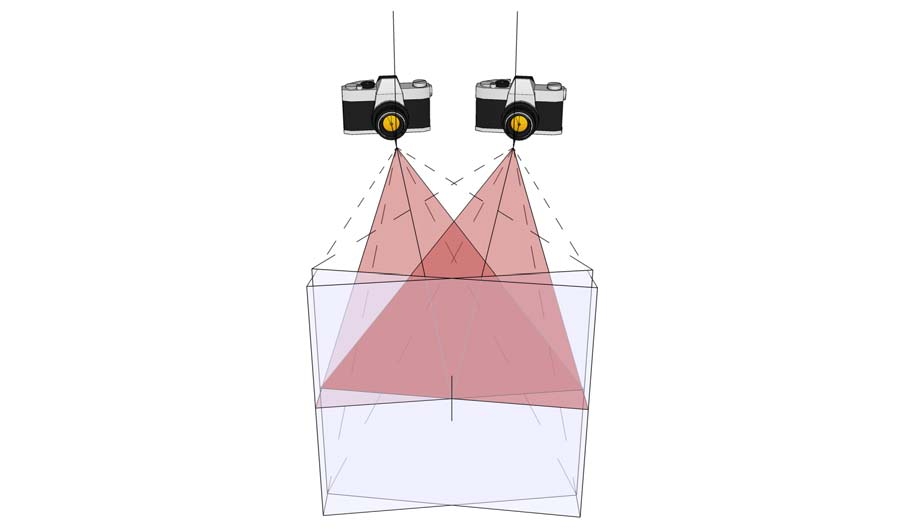
\includegraphics[width=13cm]{revisao-bibliografica/Figuras/visaocamera.png}% leia abaixo
\label{figura:figura9}

\centering \subfloat {\footnotesize { Fonte: \cite{PERONTI2008} }}
{
\label{figura:figura9}
}
\end{figure}

%\clearpage

\begin{figure}[!htb]
\caption{{\footnotesize Esquema mostrando as imagens captadas em cada olho (par estereoscópico) e a imagem resultado da fusão deste par estereoscópico \cite{PERONTI2008}.}}
 
\centering % para centralizarmos a figura
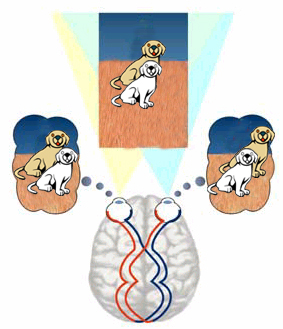
\includegraphics[width=7cm]{revisao-bibliografica/Figuras/visaohumana1.jpg}% leia abaixo
\label{figura:figura10}

\centering \subfloat {\footnotesize { Disponível em: https://i.imgur.com/Mg7u9eF.jpg }}
{
\label{figura:figura10}
}
\end{figure}
\subsection{\textbf{Captura e identificação de imagem}}

A tecnologia vem crescendo cada vez mais em todo mundo, proporcionando a ampliação do uso de dispositivos de alto desempenho. Paralelo a isso, o fluxo de dados aumenta proporcionalmente, exigindo uma velocidade de conexão maior com a Internet. Um exemplo disso são os \textit{smartphones}, que se popularizaram por serem dispositivos multifuncionais, podendo ser utilizados para tarefas profissionais e pessoais. 

Por conseguinte deste avanço científico, é notório a grande evolução na utilização de imagens digitais em várias áreas, como, por exemplo, em transmissões de TV, conteúdos via streaming, imagens capturadas por satélite e até mesmo imagens transmitidas pelas redes sociais. No entanto, como funciona a captura de uma imagem em tempo real? Qual o conceito de imagem?

Uma imagem digital pode ser considerada como sendo uma matriz de pontos elementares, em que cada ponto recebe o nome de \textit{pixel}. Quanto maior a quantidade de \textit{pixels} melhor a resolução da imagem e consequentemente maior o seu tamanho. Cada \textit{pixel} é representado por um valor que indica a intensidade de brilho, denominado nível de cinza, e a quantidade de níveis de cinza depende da quantidade de bits usada na representação de cada \textit{pixel} \cite{SOUZA2007}.

Sendo assim, a matriz de pontos elementares de uma imagem digital pode ser representada conforme na figura a seguir.

%\clearpage

%\usepackage{graphicx}
%\usepackage[portuguese]{babel} % Para termos legendas em português
\title{Figura 1} 
\date{} % para este exemplo, deixarei a data vazia
\maketitle
\begin{figure}[h]
\caption{ {\footnotesize Representação de uma imagem digital.}}
 
\centering % para centralizarmos a figura
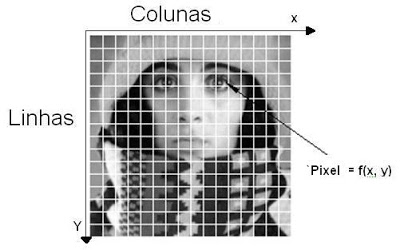
\includegraphics[width=10cm]{revisao-bibliografica/Figuras/11pixelMonocromatico.JPG} % leia abaixo
\label{figura:figura1}

\centering \subfloat {\footnotesize { Disponível em: http://sdbmcc.blogspot.com/2009/06/imagem-digital-teoria.html }}
{
\includegraphics[height=5cm]{droopy}
\label{figura:figura1}
}
\end{figure}

 
%Na Fig. \ref{figura:qualquernome}, vemos que ...


A captura e identificação em tempo real de uma imagem consiste em analisar um ambiente tridimensional e elaborar digitalmente uma imagem 2-D (Duas dimensões), ocasionando uma imagem estática daquele ambiente tridimensional selecionado. Esse conceito está relacionado a perspectiva, segundo \citeonline{PERONTI2008}. Para que isso seja possível, é necessário utilizar um dispositivo capaz de realizar essa ação, ou seja, uma câmera digital, \textit{smartphones}, dentre outros.

Segundo \citeonline{CHMIELEWSKI2009}, isso se tornou capaz devido a uma tecnologia que surgiu nos anos 70 denominada CCD, \textit{Charge Coupled Device} (Dispositivo acoplado de carga): “O sensor CCD ou dispositivo de carga acoplada é uma matriz de elementos sensíveis à luz, fabricados utilizando tecnologia MOS, \textit{Metal Oxide Semiconductor} (Semicondutor de óxido metálico), onde cada \textit{pixel} pode ser considerado como um capacitor MOS.”

Atualmente, o sensor mais utilizado nos dispositivos de captura de imagem são de sistemas digitais CMOS - \textit{Complementary Metal Oxide Semiconductor} (Semicondutor complementar de óxido metálico), que surgiu nos anos 90 devido a um protótipo do sensor de imagem APS - \textit{Active Pixel Sensor} (Sensor de pixel ativo) criado pela NASA - \textit{National Aeronautics and Space Administration} (Administração Nacional Aeronáutica e Espacial), que possibilitou a fabricação direta de funções como \textit{zoom}, diferentes resoluções de aquisições, acesso aleatório, etc., podendo executar todas as funções do CCD. “Os sensores de imagem APS são formados por elementos sensíveis à luz, capazes de gerar um sinal elétrico ou carga proporcional à intensidade da luz que incide sobre eles.” \cite{CHMIELEWSKI2009}
\subsection{\textbf{Processamento de imagem}}

De forma complementar ao assunto supracitado, o processamento de imagem evoluiu drasticamente no decorrer do avanço tecnológico. Portanto, há grande interesse nessa tecnologia pelo fato de proporcionar um grande número de aplicações, como por exemplo o aprimoramento de informações relativo a imagens para interpretação humana e análise automáticas por computador de informações extraídas da imagem capturada.

Contudo, o grande marco da área de processamento de imagens aconteceu no século XX. Com o surgimento dos primeiros computadores digitais com grande capacidade de processamento e o início do programa espacial norte-americano, ocorreu um grande impulso na área de processamento de imagem. O uso de técnicas computacionais de aprimoramento de imagens teve início no \textit{Jet Propulsion Laboratory} (Laboratório de Propulsão a Jato), localizado no centro tecnológico da NASA, em 1964, quando "imagens da lua transmitidas por uma sonda Ranger eram processadas por computador para corrigir vários tipos de distorção inerentes à câmera de TV acoplada à sonda". Essa tecnologia foi usada em grandes expedições tripuladas, como a Apollo \cite{FILHO1999}.

Para realizar o processamento de uma imagem, são definidos passos a serem seguidos para a garantia do objetivo final. A captura da imagem consiste no uso de dispositivos físicos sensíveis a espectros de energia eletromagnética que convertem o sinal elétrico para um formato digital. O pré-processamento consiste no realce da imagem para enfatizar características de interesse ou recuperar imagens que sofreram alguma degradação devido à introdução de ruído, perda de contraste ou borramento. A segmentação é a extração ou identificação dos objetos contidos na imagem, separando a imagem em regiões. Por fim, a classificação, é o processo que identifica a imagem observada \cite{GONZALEZ2002}.

As etapas básicas do processamento de imagem estão representadas através do diagrama de blocos abaixo.

\title{Figura 2} 
\date{} % para este exemplo, deixarei a data vazia
\maketitle
\begin{figure}[h]
\caption{{\footnotesize Etapas básicas do processamento de imagens.}}
 
\centering % para centralizarmos a figura
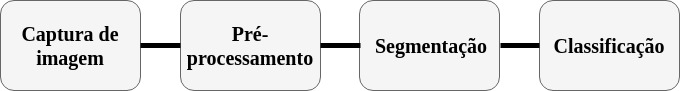
\includegraphics[width=12cm]{revisao-bibliografica/Figuras/etapas-processamento.jpg} % leia abaixo
\label{figura:figura2}

\centering \subfloat {\footnotesize { Fonte: Adaptada de \cite{GONZALEZ2002} }}
{
\includegraphics[height=5cm]{droopy}
\label{figura:figura2}
}
\end{figure}

Seres humanos conseguem distinguir vários padrões de cores com certa facilidade, levando em consideração que a análise é feita em um ambiente tridimensional. Na computação, esse discernimento de cores são mais complexos, independentemente da dimensão na qual a imagem será analisada. Isso ocorre porque vários fatores podem contribuir para a má performance computacional no tratamento da imagem, como por exemplo a falta ou excesso de luz, qualidade do sensor, qualidade da imagem, dentre outros.

\begin{quoting}[rightmargin=0cm,leftmargin=4cm]
\begin{singlespace}
{\footnotesize  
“Objetos que emitem luz visível são percebidos em função da soma das cores espectrais emitidas. Tal processo de formação é denominado aditivo. O processo aditivo pode ser interpretado como uma combinação variável em proporção de componentes monocromáticas nas faixas espectrais associadas às sensações de cor verde, vermelho e azul, as quais são responsáveis pela formação de todas as demais sensações de cores registradas pelo olho humano. Assim, as cores verde, vermelho e azul são ditas cores primárias. Este processo de geração suscitou a concepção de um modelo cromático denominado RGB (Red, Green, e Blue), para o qual a Comissão Internacional de Iluminação (CIE) estabeleceu as faixas de comprimento de onda das cores primárias.” \cite{QUEIROZ2006}
}
\end{singlespace}
\end{quoting}

Cada \textit{pixel} é representado por um valor numérico que corresponde a sua cor em questão. Sendo assim, para que seja possível representar uma imagem em alguma escala de cor monocromática (preto e branco, ou escalas de cinza), basta associar o \textit{pixel} a um valor numérico relacionado a sua escala de tom.

%\title{Figura 3} 
%\date{} % para este exemplo, deixarei a data vazia
%\maketitle
%\begin{figure}[!htb]
%\caption{Representação de cada pixel em uma imagem monocromática.}
 
%\centering % para centralizarmos a figura
%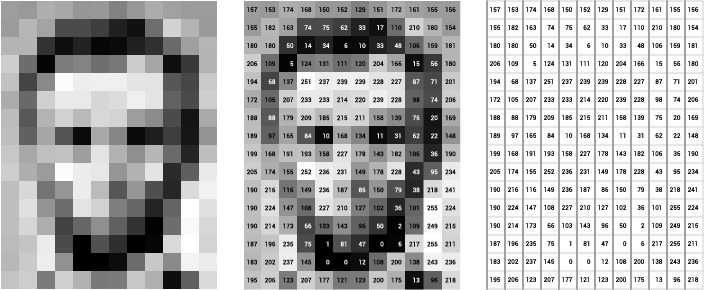
\includegraphics[width=14cm]{revisao-bibliografica/Figuras/monocromatico.jpeg}% leia abaixo
%\label{figura:figura3}

%\centering \subfloat Disponível em: https://ai.stanford.edu/~syyeung/cvweb/tutorial1.html {
%\label{figura:figura3}
%}
%\end{figure}

A figura abaixo esta exemplificando a associação dos \textit{pixels} de forma a obter uma imagem monocromática. Segundo \citeonline{NELMA2000}, para obter uma imagem em tons de cinzento, basta associar cada \textit{pixel} um valor inteiro não negativo de um byte, onde o valor 0 corresponde a cor preta e o valor máximo, 255, corresponde a cor branca. Os valores intermediários correspondem aos variados tons de cinza.

%\clearpage
%\newpage

\title{Figura 3} 
\date{} % para este exemplo, deixarei a data vazia
\maketitle
\begin{figure}[!htb]
\caption{{\footnotesize Visão computacional de \textit{pixel} monocromático.} }
 
\centering % para centralizarmos a figura
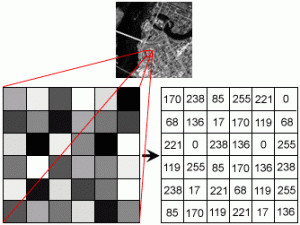
\includegraphics[width=10cm]{revisao-bibliografica/Figuras/22pixelMonocromatico.jpg}% leia abaixo
\label{figura:figura3}

\centering \subfloat {\footnotesize { Disponível em: https://ai.stanford.edu/~syyeung/cvweb/tutorial1.html }}
{
\label{figura:figura3}
}
\end{figure}


Já as imagens coloridas exigem um poder maior de processamento para serem reconhecidas. Isso ocorre porque as imagens em RGB - \textit{Red, Green, and Blue} (Vermelho, Verde e Azul)  precisam de mais de uma banda para serem processadas, ou seja, são analisadas três matrizes de cores para formar a paleta de cor específica do tom capturado. Depois da análise, são formadas as cores distintas que compõe a imagem.


\begin{figure}[H]
\caption{ {\footnotesize Matriz de \textit{pixels} RGB.}}
 
\centering % para centralizarmos a figura
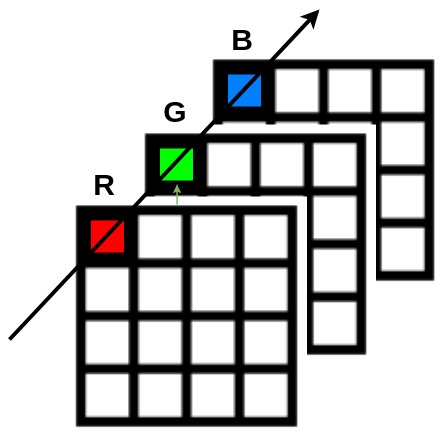
\includegraphics[width=6cm]{revisao-bibliografica/Figuras/RGB-VC.jpg}% leia abaixo
\label{figura:figura4}

\centering \subfloat {\footnotesize { Feita pelos autores do trabalho.}}
{
\label{figura:figura4}
}
\end{figure}
\FloatBarrier

De forma mais detalhada, \citeonline{LOPES2013} exemplificam que: 
\begin{quoting}[rightmargin=0cm,leftmargin=4cm]
\begin{singlespace}
{\footnotesize  
“Uma imagem colorida também é uma imagem multibanda ou multiespectral. A maioria das cores visíveis pelo olho humano pode ser representada como uma combinação de bandas das cores primárias, vermelha (R, red), verde (G, green) e azul (B, blue). Uma imagem colorida também pode ser armazenada por meio de uma imagem cromática e um mapa de cores, nesse caso, o valor de cinza de cada \textit{pixel} na imagem é considerado como um índice para uma entrada do mapa de cores, enquanto a entrada do mapa de cores contem o valor dos componentes referentes ao modelo RGB.”
}
\end{singlespace}
\end{quoting}

%\clearpage

\begin{figure}[!htb]
\caption{{\footnotesize Visão computacional de \textit{pixels} RGB.}}
 
\centering % para centralizarmos a figura
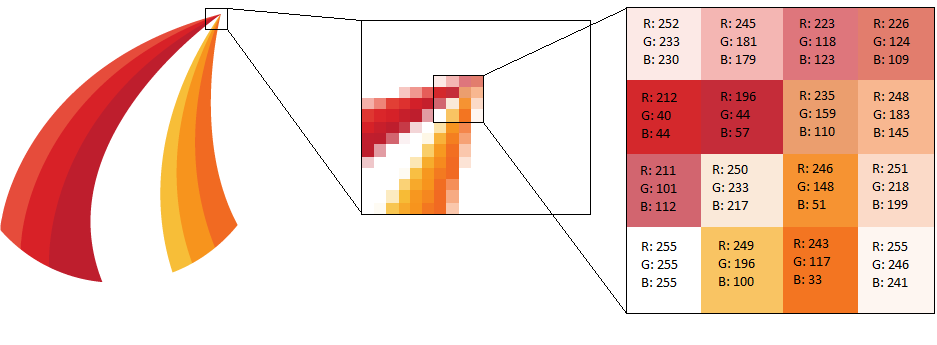
\includegraphics[width=12cm]{revisao-bibliografica/Figuras/Computer-Vision-Pixel-RGB.png}% leia abaixo
\label{figura:figura5}

\centering \subfloat {\footnotesize { Disponível em: https://www.analyticsindiamag.com/computer-vision-primer-how-ai-sees-an-image/}}
{
\label{figura:figura5}
}
\end{figure}

No entanto, a imagem capturada por algum dispositivo eletrônico pode chegar de forma irregular ate a parte de processamento. Essas falhas podem ser caracterizadas de várias formas, como por exemplo a presença de \textit{pixels} ruidosos, brilho e/ou contrastes desregulados, caracteres com dígitos incompletos ou apagados como em digitalizações de documentos.

A parte de processamento fica responsável por elaborar uma melhoria da imagem em questão, ajustando todos os parâmetros para que seja possível analisar precisamente todas as informações que estão disponíveis no arquivo de imagem. Sendo assim, por analogia as imagens processadas, trata-se de uma etapa que analisa de forma profunda todos os dados contidos na imagem, ou seja, a fase de processamento abrange os níveis mais baixos de análise de imagens, pois trabalham diretamente com valores de intensidade dos \textit{pixels}, visto que neste período não existe nenhuma informação relacionada a imagem para que seja possível facilitar o trabalho. O resultado desse processo gera imagens digitalizadas de qualidade melhor que a original.
\subsubsection{{Segmentação de imagens}}

De forma a dar continuidade ao ciclo de processamento de imagem e verificação desta, usa-se métodos de \textit{pixels} e tonalidades seguindo os padrões propostos. A análise deve prosseguir de forma minuciosa para então, processar seus detalhes.

A segmentação veio para aprimorar a parte de processamento, auxiliando na detecção de maiores detalhes e reduzindo tempo de processamento. Isso ocorre porque a segmentação é a área que tem por responsabilidade dividir a imagem em várias partes significativas, separando as de interesse dentro desta \cite{FILHO1999}.

No entanto, a segmentação exige um processamento muito grande para analisar a imagem sugerida. Sendo assim, o nível no qual será feito essa subdivisão de imagem depende muito da ocasião e do problema que está sendo proposto para resolver. De acordo com \citeonline{GONZALEZ2002}, para não ocorrer perca desnecessária de processamento e, consequentemente, perda de tempo, a segmentação deve parar assim que os objetos de interesse da aplicação forem isolados.

Portanto, dentro da segmentação existem métodos que podem ser seguidos a fim de analisar detalhadamente cada figura. Segundo \citeonline{MORGAN2008}, as classificações dos métodos utilizados na segmentação são definidos como interativos ou automáticos. Basicamente, a diferença entre os dois são bem simples: um é executado através de intervenções humanas e o outro não.

Ademais, no processo de segmentação interativa, o usuário utiliza ferramentas e técnicas que se adéquam da melhor forma a sua imagem e necessidade, solucionando-a da melhor forma possível. Esse método normalmente é mais utilizado para solucionar problemas específicos, onde as condições da imagem podem interferir drasticamente na análise final da mesma como, por exemplo, \textit{softwares} que analisam imagens de doenças graves adquiridas através de ressonâncias, onde a aplicação pode confundir um ruído ou uma área com má iluminação em um ponto de análise clínica.

Já o processo de segmentação automática onde, na maioria das vezes, utilizam robôs para realizar as tomadas de decisões através dos resultados obtidos na análise da imagem, inexiste interferência humana no processo. Esse método está sendo aplicado, por exemplo, em carros autônomos, onde o mesmo identifica a presença de obstáculos em sua frente e com base no obstáculo e na proporção do mesmo, uma ação e tomada.

Para complementar, \citeonline{MORGAN2008} enfatiza que existem métodos que são classificados de acordo com a representação dos objetos a serem segmentados, que são os métodos de borda ou orientados a regiões.

O processo de segmentação baseado no método de bordas utiliza basicamente pontos de uma imagem onde ocorre alguma intensidade de luz, ou seja, onde os \textit{pixels} estão mais visíveis, realçando a borda do objeto e consequentemente diferenciando do fundo da imagem. Pode-se também localizar uma borda através de uma mudança brusca nos tons de cinza, gerados por regiões distintas. Com base na borda que foi extraída da imagem, tem-se então uma imagem topográfica do objeto que será analisado.

A imagem a seguir mostra como funciona uma análise baseada no método de bordas.

\clearpage

\begin{figure}[!htb]
\caption{{\footnotesize Resultado de uma análise feita utilizando o método de bordas.}}
 
\centering % para centralizarmos a figura
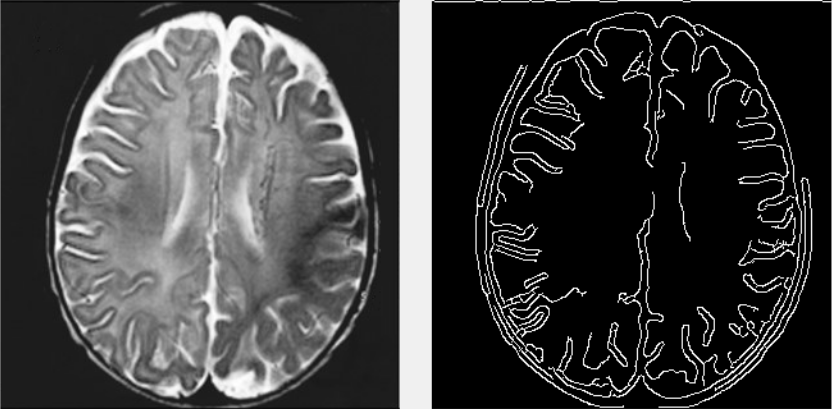
\includegraphics[width=12cm]{revisao-bibliografica/Figuras/MetodoDeBorda.png}% leia abaixo
\label{figura:figura6}

\centering \subfloat {\footnotesize { Fonte: \cite{FREITAS2016} }}
{
\label{figura:figura6}
}
\end{figure}

Conforme \citeonline{MORGAN2008} enfatiza em seu artigo, o método orientado a regiões é dividido em três abordagens relevantes: classificação por \textit{pixel}, agregação de \textit{pixel} e \textit{split-and-merge} (Divisão e conquista).

A descrever cada uma das abordagens de forma didática, a classificação por \textit{pixel} nada mais é que a identificação de características presentes na imagem como, por exemplo, cor, texturas, a fim de classificar os \textit{pixels} de acordo com as várias possibilidades de classes ou objetos da imagem.

Na abordagem de agregação por \textit{pixel} o objetivo é encontrar um \textit{pixel} dentro da imagem e, a partir desse \textit{pixel}, ocorre o crescimento de regiões conexas. O desenvolvimento das regiões acontece ate alcançar o critério de parada do crescimento, onde estará representado um objeto dentro da imagem.

Já a segmentação utilizando a bordagem \textit{split-and-merge} é mais complexa. Segundo \citeonline{VENTURA2009}, ao aplicar essa abordagem de segmentação, o objetivo final consiste em conseguir subdividir a imagem em vários quadrantes que satisfaça uma prioridade. Apos a concretização desta tarefa, realiza-se a verificação de cada quadrante, observando se este atende ou não a prioridade definida. Caso o quadrante não satisfaça a prioridade, a subdivisão acontece novamente em busca de outros quadrantes.

Por fim, o processo de fusão é realizado, acontecendo então o agrupamento das partes similares, ou seja, que atende as prioridades definidas. Esse processo só finaliza quando não existe nenhuma possibilidade de realizar divisões ou agrupamentos.
\subsubsection{{Histograma}}

De tal forma, dando continuidade ao assunto, o histograma é um método que auxilia na identificação de objetos e/ou características específicas da imagem, obtendo uma maior precisão nos resultados obtidos.

Segundo \citeonline{FILHO1999}, histograma são conjuntos de vários números no qual são indicados os percentuais de \textit{pixels} de uma imagem que possui determinados níveis de cinza. Estes valores, normalmente representados por gráficos, apresentam, para cada nível de cinza, o seu percentual de \textit{pixels} correspondente na imagem. Com base nessa análise feita pelo histograma, pode-se obter os níveis de contraste, brilho, e ate mesmo informações de predominância clara ou escura.

\begin{comment}
Para analisar cada elemento deste conjunto, \citeonline{FILHO1999} explicam, através de cálculos matemáticos, que é possível utilizando a equação a seguir:
\end{comment}

\citeonline{FILHO1999} explicam que, através de equações matemáticas, é possível obter um resultado satisfatório ao analisar cada elemento deste conjunto. Este trabalho não tem por finalidade apresentar e/ou explicar cálculos matemáticos que cada função executa.

%\begin{flalign*}
   P_r (r_k) = \frac{n_k}{n} \\
\end{flalign*}

onde:

\begin{math} 0 \le r_k \le 1 \end{math} \newline
k = 0, 1, ..., L-1, onde L é o número de níveis de cinza da imagem digitalizada; \newline
n = número total de \textit{pixels} na imagem; \newline
\begin{math} P_r (r_k) \end{math} = probabilidade do k-ésimo nível de cinza; \newline
\begin{math} n_k \end{math}= número de \textit{pixels} cujo nível de cinza corresponde a k.
 \newline

%Tabela comentada
\begin{comment}
Na tabela a seguir está sendo representado os exemplos matemáticos de histograma \cite{FILHO1999}.

\clearpage

\begin{table}[h]
\centering
\caption{{\footnotesize Exemplo de histograma.}}
\vspace{0.5cm}
\begin{tabular}{r|lr}
\hline
\hline 
Níveis de cinza (r_k) & n_k & p_r(r_k) \\ % Note a separação de col. e a quebra de linhas
\hline
\hline % para uma linha horizontal
0 & 1120    & 0,068 \\ 
1/7 & 3214  & 0,196 \\
2/7 & 4850  & 0,296 \\
3/7 & 3425  & 0,209 \\
4/7 & 1995  & 0,122 \\
5/7 & 784   & 0,048 \\
6/7 & 541   & 0,033 \\
1 & 455     & 0,028 \\  % não é preciso quebrar a última linha
\hline
\hline
Total: & 16384 & 1 \\
\hline
\hline
\end{tabular}
\end{table}
\\
\end{comment}

De forma a complementar o assunto, \citeonline{MAIZA2013} expressa em sua tese que, ao obter o histograma da imagem, pode-se alcançar medidas estatísticas dos níveis de cinza da imagem, como por exemplo o seu valor mínimo e máximo, valor médio, variância e desvio padrão. Portanto, o histograma seria como um método de probabilidade, onde o número de \textit{pixels} de um determinado nível de cinza pode ser utilizado para calcular um outro \textit{pixel} com o mesmo valor de cinza na imagem.

\begin{figure}[!htb]
\caption{ {\footnotesize Imagem (a) e seu respectivo histograma (b).}}
 
\centering % para centralizarmos a figura
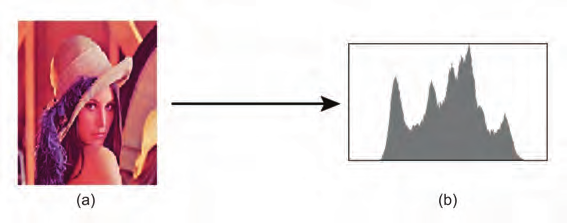
\includegraphics[width=11cm]{revisao-bibliografica/Figuras/Histograma.png}% leia abaixo
\label{figura:figura7}

\centering \subfloat {\footnotesize { Fonte: \cite{MAIZA2013} }}
{
\label{figura:figura7}
}
\end{figure}
\subsubsection{{Classificação de imagens}}
% \textbf coloca o subsection em negrito

Dentro do tema proposto, como já mencionado, a classificação de imagem é a ultima etapa do processamento de imagem. Em síntese, esta etapa é responsável por realizar a classificação das imagens levando em consideração as suas características.

Entretanto, segundo \citeonline{LIBERMAN97}, nessa etapa do processamento, o grau de abstração de cada característica da imagem podem ser classificados em três níveis distintos: baixo, médio e alto.

No processo de baixo nível são utilizados os \textit{pixels} originais da imagem como parâmetros de comparação, para que no final do processo seja gerado propriedades da imagem, em forma de valores numéricos, associados a cada \textit{pixel} que foi analisado. Sequencialmente, o nível médio coleta essas propriedades numéricas geradas pelo processo de baixo nível e produz uma lista de características da imagem. Por fim, o processo de alto nível reúne estas características ocasionadas pelo processo anterior buscando interpretá-las, formando assim o conteúdo da imagem.

Segundo \citeonline{LIBERMAN97}, o processo de classificação ou interpretação de uma imagem é a parte mais inteligente da visão computacional. O autor do artigo cita que essa é uma das etapas de maior alto nível, no qual permite-se obter a “compreensão e a descrição final do fenômeno inicial”.

Para complementar, \citeonline{LIBERMAN97} explica que o processo de classificação de imagem possui duas técnicas para realizar suas tarefas, sendo divididas em supervisionada ou não-supervisionada. A classificação não-supervisionada consiste em um agrupamento automático de sequências similares de uma imagem analisada. Conforme já prescrito neste trabalho no contexto de segmentação interativa e agora completado por \citeonline{LIBERMAN97}, nessa etapa a imagem será segmentada em um número indeterminado de classes, no qual o usuário também será responsável por gerenciar essas classes a fim de alcançar seus objetivos.

De acordo com \citeonline{MAXIMO2005}, no processo de classificação supervisionada, o analista ou usuário filtra as classes de informações seguindo os seus padrões de interesse e separa, na imagem, as regiões que satisfazem essas classes. Após a delimitação das classes, a técnica analisará as mesmas com o objetivo de delimitar \textit{pixels} que serão utilizados como parâmetros para a busca de demais \textit{pixels}.

Simplificadamente, a técnica de classificação supervisionada utiliza amostras de características coletadas durante o processo para identificar cada \textit{pixel} definido como \textit{pixel} desconhecido, ou seja, tons de \textit{pixels} que não fazem parte das características já coletadas anteriormente seguindo os filtros definidos pelo usuário.
\subsubsection{{Similaridade}}

De forma concisa, similaridade consiste em realizar uma buscar dentro de uma imagem específica com o objetivo de reconhecer/encontrar objetos semelhantes a um modelo de busca. Nessas funções de busca por similaridade são utilizados cálculos de vetores de características para realizar as comparações de igualdade \cite{MAIZA2013}.

Os seres humanos possuem uma grande facilidade de reconhecer informações apresentadas de maneira visual, onde consequentemente são capazes, com grande facilidade, de interpretar imagens diversificadas sem grande esforço. Exemplificando esta situação, os seres humanos consegue distinguir de forma fácil a diferença entre um círculo grande e um círculo pequeno, um quadrado grande de um quadrado pequeno, a diferença entre um triângulo e um quadrado de tamanhos idênticos, dentre outros. Conforme \citeonline{SILVA2009} relata em seu artigo, com a tecnologia disponível atualmente para realizar a construção de aplicações capazes de identificar informações dentro de uma imagem ainda é muito ineficiente, quando comparada com a capacidade humana.

Segundo \citeonline{MAIA2013}, algoritmos de similaridade trabalham com métricas que informam o quanto uma imagem é parecida com a outra. Ou seja, pode-se aplicar essas métricas utilizando padrões de buscas a fim de uma análise mais específica. De forma estatística, \citeonline{MAIA2013} completam que possui dois tipos básicos de medidas de similaridade: correlação e coseno. Seguindo o contexto do artigo, a similaridade por correlação entre dois vetores retorna um valor booleano, ou seja, 0 e 1, onde o valor de retorno igual a 1 significa que há uma similaridade forte naquele ponto, ou seja, os valores dos vetores são parecidos e, se o retorno for 0, não existe correlação. No entanto, o autor enfatiza a presença de um retorno igual a -1, no qual a similaridade daquele ponto é inversa ao padrão de busca. Ja a similaridade por coseno é similar a correlação, no qual o retorno também e 0 e 1, porém nesse método é analisado o tamanho do vetor e a formação de um ângulo entre os mesmos. Quanto mais próximo de 1 for o valor, mais similares são os vetores.

% Comentário de múltiplas linhas
\begin{comment}
Agregando o assunto supracitado, \citeonline{MAIZA2013}, \citeonline{MAIA2013} utilizam em seus artigos a função euclidiana para realizar cálculos de distâncias nas estruturas. Essa função utiliza métricas de similaridade para calcular a distância entre dois vetores de características, percorrendo o vetor apenas uma vez. A distância euclidiana entre dois pontos (Xi e Xj) é definida através da equação:
\end{comment}

\citeonline{MAIZA2013}, \citeonline{MAIA2013} utilizam em seus artigos a função euclidiana para realizar cálculos de distâncias nas estruturas. Essa função utiliza métricas de similaridade para calcular a distância entre dois vetores de características, percorrendo o vetor apenas uma vez. A distância euclidiana entre dois pontos (Xi e Xj) é definida através de uma equação matemática, na qual não faz parte do escopo deste projeto.

\begin{comment}

%\begin{flalign*}
   d = \sqrt{\sum_{k=1}^{n} (X_{ik} - X_{jk})^2} \\
\end{flalign*}

onde:

\begin{math} X_{ik} \end{math} e \begin{math} X_{jk} \end{math} para k = 1, e \textbf{n} as quantidades de atributos presentes nas instâncias \begin{math} X_{ik} \end{math}, \begin{math} X_{jk} \end{math}. \newline

Segundo \citeonline{MAIA2013}, a distância euclidiana necessita que quatro condições, nos vetores a, b e c, sejam validas para atuar como medida:

%\begin{enumerate}
%    \item d(a, b) \begin{math} \ge \end{math} 0;
%    \item d(a, a) = 0;
%    \item d(a, b) = d(b, a);
%    \item d(a, c) \begin{math} \le \end{math} d(a, b) + d(b, c).
%\end{enumerate}

\begin{enumerate}
    \item A distância do vetorA até o vetorB tem que ser maior ou igual a 0;
    \item A distância do vetorA até o vetorA tem que ser igual a 0, ou seja, os vetores tem que ser iguais;
    \item A distância do vetorA até o vetorB tem que ser igual a distância do vetorB até o vetorA;
    \item A distância do vetorA até o vetorC tem que ser menor ou igual a distância do vetorA até o vetorB mais a distância do vetorB até o vetorC.
\end{enumerate}

Segundo \citeonline{MAIA2013}, a distância euclidiana necessita que quatro condições nos vetores de comparação A, B e C, sejam validas para atuar como medida:

\begin{enumerate}
    \item A distância do vetorA até o vetorB tem que ser maior ou igual a 0;
    \item A distância do vetorA até o vetorA tem que ser igual a 0, ou seja, os vetores tem que ser iguais;
    \item A distância do vetorA até o vetorB tem que ser igual a distância do vetorB até o vetorA;
    \item A distância do vetorA até o vetorC tem que ser menor ou igual a distância do vetorA até o vetorB mais a distância do vetorB até o vetorC.
\end{enumerate}

O autor completa que o tamanho dos vetores influencia diretamente no desempenho da função de similaridade por distância, ou euclidiana.

\clearpage

\begin{figure}[!h]
\caption{{\footnotesize Exemplo do uso da distância Euclidiana.}}
 
\centering % para centralizarmos a figura
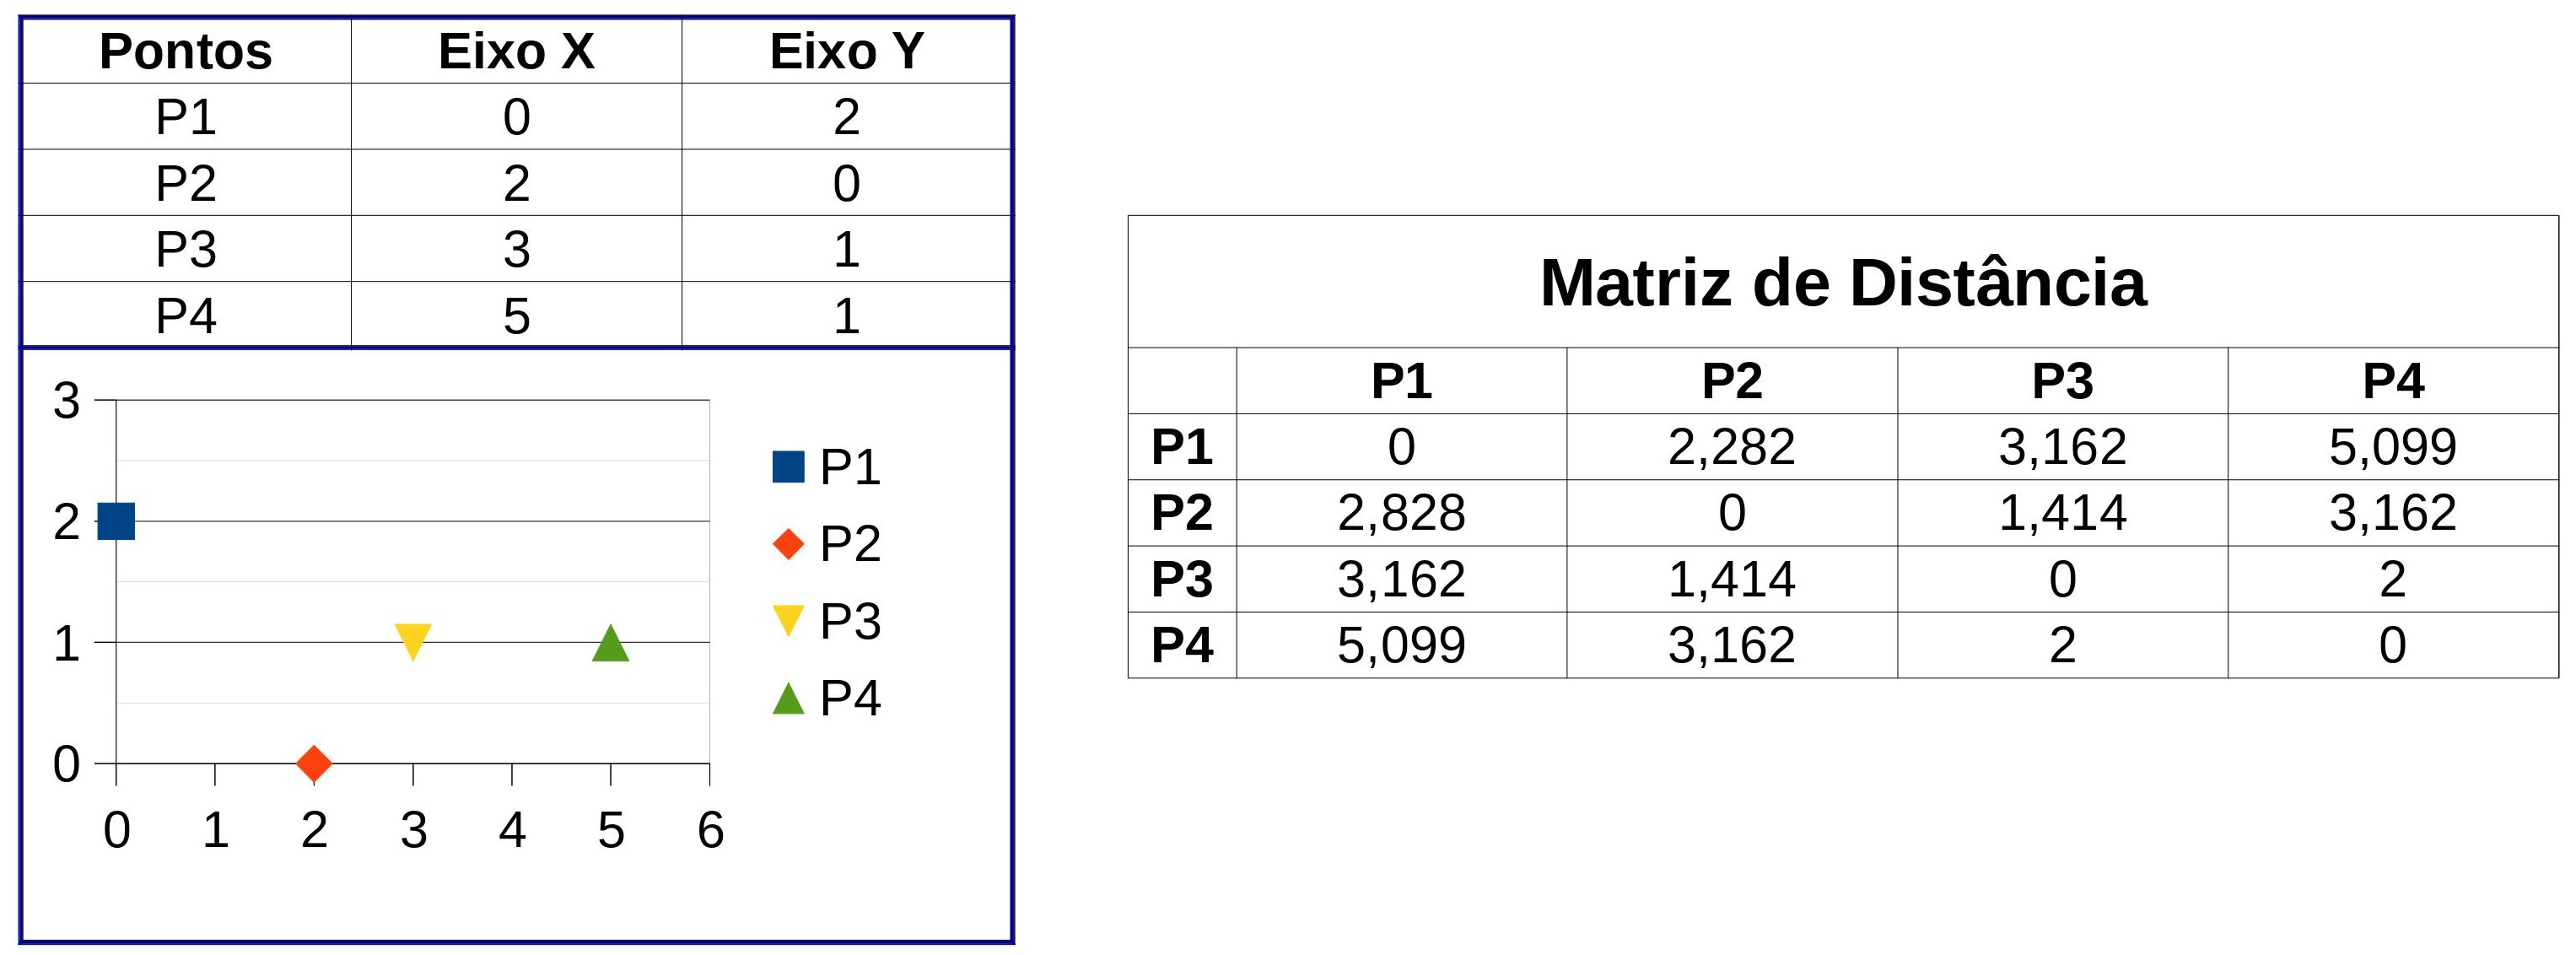
\includegraphics[width=10cm]{revisao-bibliografica/Figuras/Euclidiana.jpg}% leia abaixo
\label{figura:figura8}

\centering \subfloat {\footnotesize {Adaptado de: http://www.dsc.ufcg.edu.br/~pet/jornal/novembro2012/materias/recapitulando.html}}
{
\label{figura:figura8}
}
\end{figure}
%\clearpage
\end{comment}
\subsection{\textbf{Reconhecimento facial}}

Dentre as diversas tarefas que os computadores podem executar, o reconhecimento facial tem tido uma crescente, se tornando alvo de vários estudos. Algoritmos de reconhecimento facial estão presente em diversos dispositivos, como por exemplo \textit{smartphones} e câmeras digitais, e ate mesmo carros autônomos, que escaneiam seus obstáculos para realizar uma tomada de decisão. Grandes aperfeiçoamentos dentro desta área estão sendo implementados de forma gradativa com a finalidade de realizar análises com grandes precisões e mais próximas a visão humana.

Segundo \citeonline{SZELISKI2010}, a área de reconhecimento facial foi a que teve mais sucesso nos dias atuais. No entanto, a aplicação desse algoritmo para realizar a busca de uma pessoa dentro de milhares de pessoas em tempo real, ainda é um desafio para a tecnologia, embora pra humanos essa tarefa também é bem difícil. Mas quando esse grupo de pessoas é reduzido a, por exemplo, um grupo familiar ou grupo de amigos, a ferramenta tem um desempenho excepcional. O objeto na qual esta sentá sendo utilizado para ler o ambiente físico, ou seja, o dispositivo de captura de imagem, influencia diretamente com o desempenho da ferramenta.

Sendo assim, o resultado do reconhecimento facial pode ser intensificado quando a imagem é capturada de forma frontal as pessoas, no qual seja possível localizar por completo os rostos das pessoas em questão. Porem, vários fatores podem interferir na análise da imagem, por exemplo: iluminação, qualidade dos sensores, dentre outros fatores de interferência. Para tentar solucionar esses problemas, uma das primeiras abordagens a ser seguida pela ferramente e tentar analisar os locais de características específicas da imagem como, por exemplo, nariz, boca, olhos, e aplicar medidas de distância entre os pontos de características encontrados \cite{SZELISKI2010}.

Existem várias ferramentas que proporcionam ao usuário utilizar a tecnologia de visão computacional para realizar o reconhecimento facial. Dentre estas ferramentas, a biblioteca OpenCV disponibiliza funções capazes de reconhecer objetos e pessoas. 
\section{{FERRAMENTAS DE DESENVOLVIMENTO DO PROJETO}}

Em relação as ferramentas de desenvolvimento, é notório que existe um trajeto amplo a ser percorrido pelos programadores. Isso ocorre porque existem várias linguagens de programação e \textit{frameworks} que auxiliam no desenvolvimento de sistemas. A escolha da melhor linguagem de programação e o melhor \textit{framework} para desenvolvimento depende muito do problema a ser resolvido e também das habilidades do programador. Há também um grande impasse na escolha da melhor linguagem e/ou do melhor \textit{framework}, que está relacionado a: interesses e aplicações comerciais; comunidade, para sanar possíveis duvidas e curva de aprendizado.

\subsection{\textbf{Linguagem de programação}}

Linguagem de programação são codificações escritas sequencialmente, seguindo uma estrutura assíncrona para a resolução de algum problema ou tarefa, que tem por finalidade ser compreendida por um computador. Essas codificações descrevem ao computador a sequência lógica de execução das funções e os comandos nos quais ele deve executar para que a tarefa e/ou problema seja executado da melhor forma possível. Basicamente são divididas em linguagem de baixo nível e de alto nível, que significam, respectivamente, linguagens próximas ao entendimento de máquina ou \textit{hardware} (Binário ou hexadecimal) e linguagens próximas as linguagens naturais, ou seja, de fácil entendimento humano (\textit{While, if, write, read,} etc), nos quais são necessários compiladores para realizar a tradução, tornando possível a compreensão da máquina \cite{KELLEHER2005}.

Na busca por uma linguagem que poderia satisfazer e tornar possível a construção de uma solução para o impasse explícito no trabalho, fora identificado uma forte tendência na utilização do \textit{Python}.

\begin{comment}
De acordo com \citeonline{PILGRIM2009}, a projeção da linguagem enfatiza o trabalho do programador sobre o computacional, possibilitando assim a construção de bibliotecas e frameworks com uma facilidade acima do normal.

\textit{Python} foi criado por Guido van Rossum em 1991, com a ajuda de seus colegas Jack Jansen e Sjoerd Mullender. O objetivo deles era criar uma linguagem de fácil entendimento, orientada a objetos, menos complexa possível \cite{SONGINI2005}.

Segundo \citeonline{OLIVEIRA2007}, a linguagem sofreu vários ajustes no decorrer dos anos, tornando-se muito popular dentre os desenvolvedores e, consequentemente, dando início a enumeras aplicações. Portanto, \textit{Python} é uma linguagem orientada a objetos, fortemente tipada, com propositos gerais de alto nível e de código aberto, objetivando uma construção ágil no desenvolvimento de aplicações. Sua sintaxe e bem simples e de fácil entendimento, reduzindo o custo de manutenção em \textit{softwares} criados a partir desta. Suas bibliotecas garantem ao programador um vasto acervo de funções que tem por finalidade facilitar o seu trabalho, reduzir tempo de codificação e evitar arquivos com extensas linhas de código. Devido à comunidade de código aberto, onde desenvolvedores tem acesso ao seu código fonte, a popularização da linguagem vem crescendo de forma significativa, visto que esta ainda não é muito conhecida \cite{SONGINI2005}.
\end{comment}
\subsubsection{\textit{Python}}

De acordo com \citeonline{PILGRIM2009}, a projeção da linguagem enfatiza o trabalho do programador sobre o computacional, possibilitando assim a construção de bibliotecas e frameworks com uma facilidade acima do normal.

\textit{Python} foi criado por Guido van Rossum em 1991, com a ajuda de seus colegas Jack Jansen e Sjoerd Mullender. O objetivo deles era criar uma linguagem de fácil entendimento, orientada a objetos, menos complexa possível \cite{SONGINI2005}.

Segundo \citeonline{OLIVEIRA2007}, a linguagem sofreu vários ajustes no decorrer dos anos, tornando-se muito popular dentre os desenvolvedores e, consequentemente, dando início a enumeras aplicações. Portanto, \textit{Python} é uma linguagem orientada a objetos, fortemente tipada, com propositos gerais de alto nível e de código aberto, objetivando uma construção ágil no desenvolvimento de aplicações. Sua sintaxe e bem simples e de fácil entendimento, reduzindo o custo de manutenção em \textit{softwares} criados a partir desta. Suas bibliotecas garantem ao programador um vasto acervo de funções que tem por finalidade facilitar o seu trabalho, reduzir tempo de codificação e evitar arquivos com extensas linhas de código. Devido à comunidade de código aberto, onde desenvolvedores tem acesso ao seu código fonte, a popularização da linguagem vem crescendo de forma significativa, visto que esta ainda não é muito conhecida \cite{SONGINI2005}.
\subsection{\bf Framework}

Atualmente, os projetos de desenvolvimento de \textit{software} aumentou consideravelmente. Devido a isso, programadores se deparam com um excesso de funções similares dentro dos vários projetos desenvolvidos no decorrer do tempo. Sendo assim, surgiu a necessidade de reutilizar códigos para poupar tempo. 

De acordo com \citeonline{JOHNSON97}, \textit{framework} são estruturas desenvolvidas com o objetivo de reutilizar tudo ou parte de um sistema representado por um conjunto de classes abstratas e concretas, ou seja,  uma estrutura parcialmente completa projetada para ser instanciada. Existe também \textit{frameworks}  que disponibilizam \textit{templates} como base para iniciar o desenvolvimento.

Os \textit{frameworks} disponibilizam para os desenvolvedores um vasto conjunto de bibliotecas, permitindo assim a realização de operações de grande porte. Sendo assim, os programadores focam mais em resolver problemas do que reescrever códigos, aumentando consideravelmente a produtividade da equipe. 
\subsection{\textbf{Biblioteca \textit{OpenCV}}}

Devido aos avanços em estudos científicos tecnológicos na área de visão computacional, o surgimento de bibliotecas que utilizam desta tecnologia evoluiu consideravelmente, proporcionando aos usuários maior versatilidade na escolha da melhor ferramenta para uma possível solução de seus problemas. Dentre as principais ferramentas que implementam algoritmos de visão computacional, pode-se citar as mais utilizadas: \textit{Matlab}, \textit{OpenCV} e \textit{scikit-image}. Este trabalho tem o objetivo de abordar apenas a biblioteca \textit{OpenCV}, no qual será utilizada para o desenvolvimento de uma possível resolução ao problema supracitado. A biblioteca \textit{Open Source} (Código aberto) está disponível no seu site oficial \citeonline{OpenCV}.

Desenvolvida pela Intel no ano 2000, escrita nativamente em C++, a biblioteca OpenCV permite a manipulação de dados de imagens, manipulações vetoriais, rotinas de álgebra linear, desenvolvimento de algoritmos de processamento de imagem, calibração de câmeras, dentre outros. Sua flexibilidade com várias linguagens de programação, como por exemplo o \textit{Python}, permite uma melhor integração com vários programas, evitando possíveis conflitos de incompatibilidade e proporcionando uma melhor flexibilidade no desenvolvimento de \textit{softwares} \cite{BARBOZA2009}.

A bilioteca possui certificação BSD - \textit{Berkeley Software Distribution}, representando que o software possui uma licença gratuita. A biblioteca contem mais de 2.500 algoritmos otimizados com diversas propriedades para resolverem problemas extensos. Há também vários setores de aplicação da biblioteca, visto que esta abrange diversas áreas como, por exemplo, reconhecimento de face e objetos, extração de modelos de objetos tridimensionais, união de imagens em uma única imagem, pesquisar por imagens semelhantes dentro de um banco de dados, acompanhar movimentos dos olhos, reconhecimento de cenários, dentre outros. No site oficial da ferramenta encontra-se dados nos quais informam que esta possui uma comunidade com mais de 47 mil usuários e um número estimado de download que ultrapassa a casa dos 18 milhões \cite{CUNHA2013}.

Segundo \citeonline{CUNHA2013}, um dos objetivos da biblioteca \textit{OpenCV} é fornecer uma infraestrutura robusta na área de visão computacional na qual seja de fácil manipulação, ajudando os desenvolvedores no processo de ampliação de aplicações sofisticadas de visão.
\subsection{\textbf{Sistema de controle de versões}}

Durante o processo de desenvolvimento de \textit{software}, a etapa de codificação gera várias linhas de códigos. Além disso, modificações e melhorias no \textit{software} ocorrem constantemente no decorrer do tempo, seja a pedido do usuário ou alguma possível atualização.  As equipes de desenvolvimento são compostas por vários tipos de desenvolvedores, cada um com sua personalidade e experiência. Sendo assim, os desenvolvimentos de \textit{softwares} são feitos por etapas, onde cada desenvolvedor é responsável por entregar o que foi designado a ele. 

Devido a isso, para organizar essas etapas de desenvolvimento, utiliza-se ferramentas gerencia e controla diferentes versões de \textit{software}.  Segundo \citeonline{OReilly},  uma ferramenta que realiza o gerenciamento e o controle de versões de \textit{software} ou outro conteúdo “é referida genericamente como um VCS - \textit{Version Control System} (Sistema de controle de versão ), um SCM - \textit{Source Code Manager} (Gerenciador de código-fonte) ou um RCS - \textit{Revision Control System} (Sistema de controle de revisão)”. Essas ferramentas controlam quais linhas de códigos foram alteradas, qual contribuidor do projeto fez a alteração, o horário da alteração, dentre outros. Além do mais, essas ferramentas possibilitam aos desenvolvedores uma opção de voltar o código para versões anteriores, caso algum \textit{bug} (Problema) na versão atual do sistema cause algum transtorno.

\citeonline{OReilly} enfatizam que nenhuma pessoa criativa e cautelosa inicia um projeto sem um método de \textit{backup}. Sendo assim, outra funcionalidade muito importante que as ferramentas de rastreamento e gerenciamento de código proporcionam para os desenvolvedores são os repositórios de \textit{backup}, que mantêm hospedado de forma segura todas os arquivos relacionados ao sistema desenvolvido.
%\subsection{\textbf{\textit{Haar Cascade}}}
\subsubsubsection{\textit{Haar Cascade}}

Para complementar o assunto citado acima, a técnica de \textit{Haar Cascade} utiliza a classificação de imagens para obter um padrão de características que foram extraídas da imagem. Essa classificação é utilizada para montar uma cascata de características, ou seja, um conjunto de imagens. A principal base para a detecção de objetos do classificador \textit{Haar} são os recursos extraídos da imagem, ou seja, ao invés de usar os valores de intensidade de um \textit{pixel}, usa-se as alterações nos valores de contraste entre os grupos retangulares dos \textit{pixels}. Basicamente, \textit{Haar Cascade} é baseada em \textit{Haar Wavelets}, que utiliza uma sequência de funções redimensionadas em quadrantes que juntas formam uma base de \textit{wavelets} \cite{WILSON2006}.

A detecção de objetos e faces utilizando técnicas de classificadores em cascata baseados em recursos \textit{Haar} é um método eficaz proposto por \citeonline{VIOLA2001} em seu artigo. Á abordagem é baseada em \textit{machine learning} (aprendizado de máquina) no qual a função cascata é treinada a partir de enumeras imagens positivas e negativas. Através desse recurso, pode-se obter a eficiência em detecção de objetos em outras imagens \cite{OpenCV}. Este trabalho não descreve os detalhes do funcionamento do detector de Viola-Jones. O leitor interessado pode encontrá-lo em \cite{VIOLA2001}.
\subsection{\textbf{\textit{Machine Learning}}}
\section{{DESENVOLVIMENTO ÁGIL DE \textit{SOFTWARE}}}

Quando se pensa em desenvolvimento de \textit{software}, deve-se reconhecer que o processo é bem instável e com baixa previsibilidade, se tornando algo complicado de estabelecer métricas a serem seguidas. Vários pontos de interferência pode intervir para que um \textit{software} não possa ser desenvolvido da maneira correta, como por exemplo uma má equipe de trabalho, nos quais os integrantes não possuem uma boa convivência entre si, ou uma má metodologia de desenvolvimento sem uma linha cronológica a ser seguida. Reconhecer que este é um grande desafio é algo sensato de se fazer. No entanto existem mecanismos de correção para melhorar o processo de desenvolvimento.

A metodologia ágil surgiu para organizar esses processos de desenvolvimento de \textit{software}, elaborando uma padronização nos projetos para que seja possível otimizar os fluxos de trabalho e melhoras a produtividade do projeto. Segundo \citeonline{SOARES2004}, a principal característica da metodologia ágil e que ela pode ser adaptada, ao invés de ser preditiva. Ou seja, se ocorrer algum problema no decorrer do desenvolvimento, a própria metodologia é flexível o bastante para contornar a situação e prosseguir com o desenvolvimento do projeto. Portanto, uma empresa pode facilmente criar a sua própria metodologia de trabalho, seguindo a sua experiência empresarial, analisando os seus acertos e erros para elaborar um procedimento que se adéqua as suas necessidades. 

\citeonline{SOARES2004} continua exemplificando que a metodologia ágil trabalha com constantes \textit{feedbacks} e reuniões, nas quais permitem aos membros da equipe expor as facilidades e dificuldades de suas tarefas, bem como o seu status de desenvolvimento. A partir destes \textit{feedbacks}, o gestor pode traçar a melhor maneira de organizar a equipe para que os membros com maior experiência deem apoio nas dificuldades apresentadas pelos outros integrantes da equipe. Outro grande motivo expressado no contexto é o fato ocorrer entregas constantes de partes operacionais do software. Desta maneira, o usuário final do software pode ter uma prévia de como o sistema está sendo desenvolvido, bem como suas funcionalidades e \textit{design}, podendo solicitar alguma possível alteração ou identificar algum problema antes da implantação oficial dos modulos.


\subsection{\textbf{\textit{Kanban}}}

De forma a complementar o assunto, o \textit{Kanban} é um método ágil de desenvolvimento de software que permite a interação de várias áreas e membros do projeto por meio de cartões que contem o progresso de cada atividade. Cada cartão contem uma instrução a ser seguida pela área ou pelo integrante no qual foi designado para a atividade. Sendo assim, seu principal foco e fornecer um trabalho progressivo, apresentando as evoluções e dificuldades de forma clara e transparente, favorecendo uma cultura de melhoria contínua \cite{KANBAN2014}.

Sendo assim, o \textit{Kanban} tem um grande potencial em trabalho conjunto para a finalização de um item em especifico, justamente para que não ocorra nenhum gargalo na entrega de um item essencial para o trabalho do integrante ou da área seguinte. Outra grande característica é evitar ou diminuir o índice de trabalhos repetitivos que, por um eventual descuido, possa acontecer de desenvolvedores realizarem a mesma codificação de uma mesma função ou \textit{API - Application Programming Interface} (Interface de Programação de Aplicações), por exemplo.

O \textit{Kanban} foi criado pelo vice presidente da \textit{Toyota Motor Company}, o sr. Taiichi Ohno, no qual teve como principal objetivo o aumento do valor agregado entregue nas atividades de cada colaborador de sua equipe. Com este pensamento,  Ohno concluiu que as pilhas de materiais estocados e as filas de de espera era um “dinheiro parado” que a empresa \textit{Toyota} estava desperdiçando. Portando,   Ohno uniu os princípios do método \textit{just in time} (Determina que tudo deve ser feito na hora exata)  juntamente com o \textit{Jidoka} (Determina que corrigir o problema em si não é o bastante, e sim corrigir a origem do problema) para elaborar um metodo mais aprimorado de organização dentro da empresa \textit{Toyota}, denominado \textit{Kanban} \cite{TOYOTA1977}.

Atualmente, a metodologia ágil \textit{Kanban} é utilizada em diversas empresas para realizar o controle de desempenho de diversas área de atuação.
\subsection{\textbf{\textit{Trello}}}
%\input{./revisao-bibliografica/modelo.tex}
%\chapter{DESENVOLVIMENTO}

Neste capítulo aborda todo o processo utilizado para o desenvolvimento desse projeto...

\section{DESCRIÇÃO DO SISTEMA}

O QUE O SOFTWARE VAI FAZER
\subsection{\textbf{Etapas de funcionamento}}
COMO ELE VAI FAZER
\section{{DESENVOLVIMENTO DO SISTEMA}}

COMO FOI FEITO
\subsection{\textbf{Requisitos funcionais}}
\subsection{\textbf{Requisitos não-funcionais}}
\section{{AMBIENTE DE TESTES}}

\pagebreak
\chapter{METODOLOGIA}

A metodologia utilizada no projeto é a exploratória.

Segundo \citeonline{VENTURA2007}, são verificadas grandes utilidades em estudos de casos realizados através de pesquisas exploratórias.

\begin{quoting}[rightmargin=0cm,leftmargin=4cm]
\begin{singlespace}
{\footnotesize  
“Por sua flexibilidade, é recomendável nas fases iniciais de uma investigação sobre temas complexos, para a construção de hipóteses ou reformulação do problema. Também se aplica com pertinência nas situações em que o objeto de estudo já é suficientemente conhecido a ponto de ser enquadrado em determinado tipo ideal. São úteis também na exploração de novos processos ou comportamentos, novas descobertas, porque têm a importante função de gerar hipóteses e construir teorias. Ou ainda, pelo fato de explorar casos atípicos ou extremos para melhor compreender os processos típicos.”
}
\end{singlespace}
\end{quoting}

Este estudo tem por finalidade apresentar resultados qualitativos sobre o assunto de visão computacional, visando explorar a didática e o conteúdo metodológico relacionado similarmente à pesquisa.

A pesquisa qualitativa será realizada baseada no livro \textit{Digital Image Processing} \cite{GONZALEZ2002}. Este livro fora escolhido para transmitir o conceito científico e teórico sobre o assunto de visão computacional. O segundo livro que será utilizado para extrair maiores informações sobre o assunto é o Processamento Digital de Imagens \cite{FILHO1999}, que também aborda conteúdos didáticos e científicos sobre o assunto, explicando a funcionalidade da visão computacional, como esta trabalha e a resolução dos problemas sucintos.

Outro livro que será utilizado para a síntese de informações é o \textit{Computer Vision: Algorithms and Applications} \cite{SZELISKI2010}, que cita relações sobre o assunto de forma clara e objetiva.

Portanto, a pesquisa relacionada ao tema desse trabalho será baseada em todos os livros descritos e alguns artigos, com a finalidade de desenvolver o conteúdo teórico sobre o assunto de forma à fácil entendimento.
%% Orientação paisagem
%\begin{landscape}

\chapter{CRONOGRAMA}

\begin{enumerate}
\item \label{1} Elaboração da proposta de TCC.
\item \label{2} Análise/Pesquisa sobre o tema Visão Computacional.
\item \label{3} Apresentação da pesquisa sobre o tema Visão Computacional.
\item \label{4} Desenvolvimento da aplicação. 
\item \label{5} Elaboração da parte escrita.
\item \label{6} Defesa e revisão do trabalho.
\end{enumerate}

\definecolor{midgray}{gray}{0.6}
\definecolor{nocolor}{gray}{1}

\centering
\begin{table}[!htb]
\centering
\begin{tabular}{|c|c|c|c|c|c|c|c|c|c|c|c|c|c|c|c|c|c|c|c|c|c|c|}
\hline
\multirow{2}{}{}&\multicolumn{22}{c|}{2019}\\\cline{2-23}
&\multicolumn{2}{c|}{FEV}&\multicolumn{2}{c|}{MAR}&\multicolumn{2}{c|}{ABR}&\multicolumn{2}{c|}{MAI}&\multicolumn{2}{c|}{JUN}&\multicolumn{2}{c|}{JUL}&\multicolumn{2}{c|}{AGO}&\multicolumn{2}{c|}{SET}&\multicolumn{2}{c|}{OUT}&\multicolumn{2}{c|}{NOV}&\multicolumn{2}{c|}{DEZ}\\
\hline
\ref{1}&\cellcolor{midgray}\textcolor{midgray}{x}&\cellcolor{midgray}\textcolor{midgray}{x}&\cellcolor{midgray}\textcolor{midgray}{x}&\cellcolor{midgray}\textcolor{midgray}{x}&\cellcolor{nocolor}\textcolor{nocolor}{y}&\cellcolor{nocolor}\textcolor{nocolor}{y}&\cellcolor{nocolor}\textcolor{nocolor}{y}&\cellcolor{nocolor}\textcolor{nocolor}{y}&\cellcolor{nocolor}\textcolor{nocolor}{y}&\cellcolor{nocolor}\textcolor{nocolor}{y}&\cellcolor{nocolor}\textcolor{nocolor}{y}&\cellcolor{nocolor}\textcolor{nocolor}{y}&\cellcolor{nocolor}\textcolor{nocolor}{y}&\cellcolor{nocolor}\textcolor{nocolor}{y}&\cellcolor{nocolor}\textcolor{nocolor}{y}&\cellcolor{nocolor}\textcolor{nocolor}{y}&\cellcolor{nocolor}\textcolor{nocolor}{y}&\cellcolor{nocolor}\textcolor{nocolor}{y}&\cellcolor{nocolor}\textcolor{nocolor}{y}&\cellcolor{nocolor}\textcolor{nocolor}{y}&\cellcolor{nocolor}\textcolor{nocolor}{y}&\cellcolor{nocolor}\textcolor{nocolor}{y}\\
\hline

\ref{2}&\cellcolor{nocolor}\textcolor{nocolor}{x}&\cellcolor{nocolor}\textcolor{nocolor}{x}&\cellcolor{midgray}\textcolor{midgray}{x}&\cellcolor{midgray}\textcolor{midgray}{x}&\cellcolor{midgray}\textcolor{midgray}{x}&\cellcolor{midgray}\textcolor{midgray}{x}&\cellcolor{midgray}\textcolor{midgray}{x}&\cellcolor{midgray}\textcolor{midgray}{x}&\cellcolor{midgray}\textcolor{midgray}{y}&\cellcolor{midgray}\textcolor{midgray}{y}&\cellcolor{nocolor}\textcolor{nocolor}{y}&\cellcolor{nocolor}\textcolor{nocolor}{y}&\cellcolor{nocolor}\textcolor{nocolor}{y}&\cellcolor{nocolor}\textcolor{nocolor}{y}&\cellcolor{nocolor}\textcolor{nocolor}{y}&\cellcolor{nocolor}\textcolor{nocolor}{y}&\cellcolor{nocolor}\textcolor{nocolor}{y}&\cellcolor{nocolor}\textcolor{nocolor}{y}&\cellcolor{nocolor}\textcolor{nocolor}{y}&\cellcolor{nocolor}\textcolor{nocolor}{y}&\cellcolor{nocolor}\textcolor{nocolor}{y}&\cellcolor{nocolor}\textcolor{nocolor}{y}\\
\hline

\ref{3}&\cellcolor{nocolor}\textcolor{nocolor}{x}&\cellcolor{nocolor}\textcolor{nocolor}{x}&\cellcolor{nocolor}\textcolor{nocolor}{x}&\cellcolor{nocolor}\textcolor{nocolor}{x}&\cellcolor{nocolor}\textcolor{nocolor}{x}&\cellcolor{nocolor}\textcolor{nocolor}{x}&\cellcolor{nocolor}\textcolor{nocolor}{x}&\cellcolor{nocolor}\textcolor{nocolor}{x}&\cellcolor{nocolor}\textcolor{nocolor}{y}&\cellcolor{nocolor}\textcolor{nocolor}{y}&\cellcolor{midgray}\textcolor{midgray}{y}&\cellcolor{nocolor}\textcolor{nocolor}{y}&\cellcolor{nocolor}\textcolor{nocolor}{y}&\cellcolor{nocolor}\textcolor{nocolor}{y}&\cellcolor{nocolor}\textcolor{nocolor}{y}&\cellcolor{nocolor}\textcolor{nocolor}{y}&\cellcolor{nocolor}\textcolor{nocolor}{y}&\cellcolor{nocolor}\textcolor{nocolor}{y}&\cellcolor{nocolor}\textcolor{nocolor}{y}&\cellcolor{nocolor}\textcolor{nocolor}{y}&\cellcolor{nocolor}\textcolor{nocolor}{y}&\cellcolor{nocolor}\textcolor{nocolor}{y}\\
\hline

\ref{4}&\cellcolor{nocolor}\textcolor{nocolor}{x}&\cellcolor{nocolor}\textcolor{nocolor}{x}&\cellcolor{nocolor}\textcolor{nocolor}{x}&\cellcolor{nocolor}\textcolor{nocolor}{x}&\cellcolor{nocolor}\textcolor{nocolor}{y}&\cellcolor{nocolor}\textcolor{nocolor}{y}&\cellcolor{nocolor}\textcolor{nocolor}{y}&\cellcolor{nocolor}\textcolor{nocolor}{y}&\cellcolor{nocolor}\textcolor{nocolor}{y}&\cellcolor{midgray}\textcolor{midgray}{y}&\cellcolor{midgray}\textcolor{midgray}{y}&\cellcolor{midgray}\textcolor{midgray}{y}&\cellcolor{midgray}\textcolor{midgray}{y}&\cellcolor{midgray}\textcolor{midgray}{y}&\cellcolor{midgray}\textcolor{midgray}{y}&\cellcolor{midgray}\textcolor{midgray}{y}&\cellcolor{midgray}\textcolor{midgray}{y}&\cellcolor{nocolor}\textcolor{nocolor}{y}&\cellcolor{nocolor}\textcolor{nocolor}{y}&\cellcolor{nocolor}\textcolor{nocolor}{y}&\cellcolor{nocolor}\textcolor{nocolor}{y}&\cellcolor{nocolor}\textcolor{nocolor}{y}\\
\hline

\ref{5}&\cellcolor{nocolor}\textcolor{nocolor}{x}&\cellcolor{nocolor}\textcolor{nocolor}{x}&\cellcolor{nocolor}\textcolor{nocolor}{x}&\cellcolor{nocolor}\textcolor{nocolor}{x}&\cellcolor{nocolor}\textcolor{nocolor}{y}&\cellcolor{nocolor}\textcolor{nocolor}{y}&\cellcolor{nocolor}\textcolor{nocolor}{y}&\cellcolor{nocolor}\textcolor{nocolor}{y}&\cellcolor{nocolor}\textcolor{nocolor}{y}&\cellcolor{nocolor}\textcolor{nocolor}{y}&\cellcolor{nocolor}\textcolor{nocolor}{y}&\cellcolor{midgray}\textcolor{midgray}{y}&\cellcolor{midgray}\textcolor{midgray}{y}&\cellcolor{midgray}\textcolor{midgray}{y}&\cellcolor{midgray}\textcolor{midgray}{y}&\cellcolor{midgray}\textcolor{midgray}{y}&\cellcolor{midgray}\textcolor{midgray}{y}&\cellcolor{midgray}\textcolor{midgray}{y}&\cellcolor{midgray}\textcolor{midgray}{y}&\cellcolor{midgray}\textcolor{midgray}{y}&\cellcolor{nocolor}\textcolor{nocolor}{y}&\cellcolor{nocolor}\textcolor{nocolor}{y}\\
\hline

\ref{6}&\cellcolor{nocolor}\textcolor{nocolor}{x}&\cellcolor{nocolor}\textcolor{nocolor}{x}&\cellcolor{nocolor}\textcolor{nocolor}{x}&\cellcolor{nocolor}\textcolor{nocolor}{x}&\cellcolor{nocolor}\textcolor{nocolor}{y}&\cellcolor{nocolor}\textcolor{nocolor}{y}&\cellcolor{nocolor}\textcolor{nocolor}{y}&\cellcolor{nocolor}\textcolor{nocolor}{y}&\cellcolor{nocolor}\textcolor{nocolor}{y}&\cellcolor{nocolor}\textcolor{nocolor}{y}&\cellcolor{nocolor}\textcolor{nocolor}{y}&\cellcolor{nocolor}\textcolor{nocolor}{y}&\cellcolor{nocolor}\textcolor{nocolor}{y}&\cellcolor{nocolor}\textcolor{nocolor}{y}&\cellcolor{nocolor}\textcolor{nocolor}{y}&\cellcolor{nocolor}\textcolor{nocolor}{y}&\cellcolor{nocolor}\textcolor{nocolor}{y}&\cellcolor{nocolor}\textcolor{nocolor}{y}&\cellcolor{nocolor}\textcolor{nocolor}{y}&\cellcolor{nocolor}\textcolor{nocolor}{y}&\cellcolor{midgray}\textcolor{midgray}{y}&\cellcolor{midgray}\textcolor{midgray}{y}\\
\hline
\end{tabular}
\end{table}

%\end{landscape}

\pagebreak
\chapter{DESENVOLVIMENTO}

Neste capítulo aborda todo o processo utilizado para o desenvolvimento desse projeto...

\section{DESCRIÇÃO DO SISTEMA}

O QUE O SOFTWARE VAI FAZER
\subsection{\textbf{Etapas de funcionamento}}
COMO ELE VAI FAZER
\section{{DESENVOLVIMENTO DO SISTEMA}}

COMO FOI FEITO
\subsection{\textbf{Requisitos funcionais}}
\subsection{\textbf{Requisitos não-funcionais}}
\section{{AMBIENTE DE TESTES}}

\pagebreak
\chapter{CONSIDERAÇÕES FINAIS}

Escreva aqui as conclusões deste trabalho, lembrando que os objetivos geral e específicos devem ser citados e comentados,  ou seja, descreva como cada objetivo foi alcançado.

\section{{ANÁLISE DOS RESULTADOS}}
\section{{PROPOSTAS DE NOVOS ESTUDOS}}

\pagebreak
%\def\bibname{REFERÊNCIAS}
\settocbibname{REFERÊNCIAS}
\bibliography{refbib}

\pagebreak
% O * remove o indice do capítulo no sumário
\chapter*{GLOSSÁRIO}
% A função \addcontentsline coloca um capítulo sem indice no sumário
\addcontentsline{toc}{chapter}{GLOSSÁRIO}

% O * remove o indice do capítulo no sumário
\chapter*{ANEXO}
\addcontentsline{toc}{chapter}{ANEXO}


\end{document}